\documentclass[a4paper,12pt]{article}
\usepackage{czech}
\usepackage[utf8]{inputenc}
\usepackage{a4wide}
\usepackage[dvipdfm]{graphicx}
\usepackage{graphics}
\usepackage{indentfirst}
\usepackage{fancyhdr}
\usepackage{setspace}
\usepackage{amsmath}
\usepackage{amssymb}
\usepackage{epsfig}

%%\usepackage{nopageno}
%%\usepackage{txfonts}
\usepackage[usenames]{color}

\begin{document}
\newcommand{\st}{^{\circ}}
\newcommand{\RJ}{\mbox{RJ}}
\newcommand{\mV}{\mbox{m}/\mbox{V}^2}

\section{Úkol}
\begin{enumerate}
    \item Sestavte aparaturu pro sledování příčného elektrooptického jevu v pevném vzorku. Laser umístěte tak, aby byl zdroj světla polarizován kolmo k vodorovné rovině. (Předem najděte směr snadného průchodu polarizátorů používaných v aparatuře).
    \item Změřte závislost intenzity světla dopadající na detektor na napětí přiloženém na elektrody vzorku (nepřekračujte 1kV !). Zpracujte graficky.

    \item Ze směrnice závislosti fázového posunu mezi řádným a mimořádným paprskem na čtverci přiloženého napětí určete Kerrovu konstantu vzorku. Určete půlvlnné napětí.
    \item Diskutujte vliv nepřesnosti parametrů $d$ a $l$ na výsledky měření. Zvažte vhodnou oblast pro fitování výsledků.
    \item Změřte závislost fázového posunu na napští na elektrodách za pomoci proměnné polohy analyzátoru.
\end{enumerate}
 

\section{Teorie}
\subsection{Brewsterův úhel}
Při dopadu paprsku na opticky hustší prostředí pod úhlem $\theta_B$, který splňuje rovnici
\begin{eqnarray}
\tan\theta_B=\frac{n_2}{n_1}
\label{Brew}
\end{eqnarray}
dochází k polarizaci odrazem. Odražený paprsek je polarizován v rovině kolmé na rovinu dopadu. Detaily naleznete v \cite{maly}.

\subsection{Kerrův jev v pevné látce}
Kerrův jev je ve zkratce posun roviny polarizovaného světla po průchodu látkou. Tento jev je závislý na mimo rozměrů látky na čtverci elektrické intenzity uvnitř. 
Přesný vztah pro fázový posun je
\begin{eqnarray}
\Delta=2\pi KlE^2,
\end{eqnarray}
kde $K$ je Kerrova konstanta, $l$ délka vzorku a $E$ elektrická intenzita.
Při použití pole vytvořeným za pomoci napětí přivedeném na elektrody ve vzorku, které jsou od sebe ve vzdálenosti $d$ pro intenzitu světla prošlým zkříženými polarizačnímy 
filtry mezi kterými je vzorek platí
\begin{eqnarray}
I=I_0\sin^2\frac{\pi KlU^2}{d^2}.
\label{I}
\end{eqnarray}
Tento vztah se dá upravit na
\begin{eqnarray}
U^2=\frac{d^2}{\pi Kl}\arcsin\sqrt{\frac{I}{I_0}},
\label{Kb}
\end{eqnarray}
který je dále používán pro určení Kerrovy konstanty, kdy se dopočítá ze směrnice závislosti kvadrátu napětí na fázovém posunu.

\section{Měření}
\subsection{Stanovení směru snadného prlchodu polarizátoru}
Sestavil jsem aparaturu dle obrázku \ref{Obr1}. Pro skleněnou destičku jsem bral index lomu $n=1.5$. Z toho plyne dle \ref{Brew}, že
\begin{eqnarray}
\alpha_B=56.3\st.
\end{eqnarray}
Minimum intenzity světla byla u obou polarizátorů v okolí nuly. V zhledem k mělkosti tohoto minima a subjektivnosti oka nejsem sto stanovit přsnou hodnotu. 
Minimum mělo šířku přibližně $3\st$.

\begin{figure}
\begin{center}
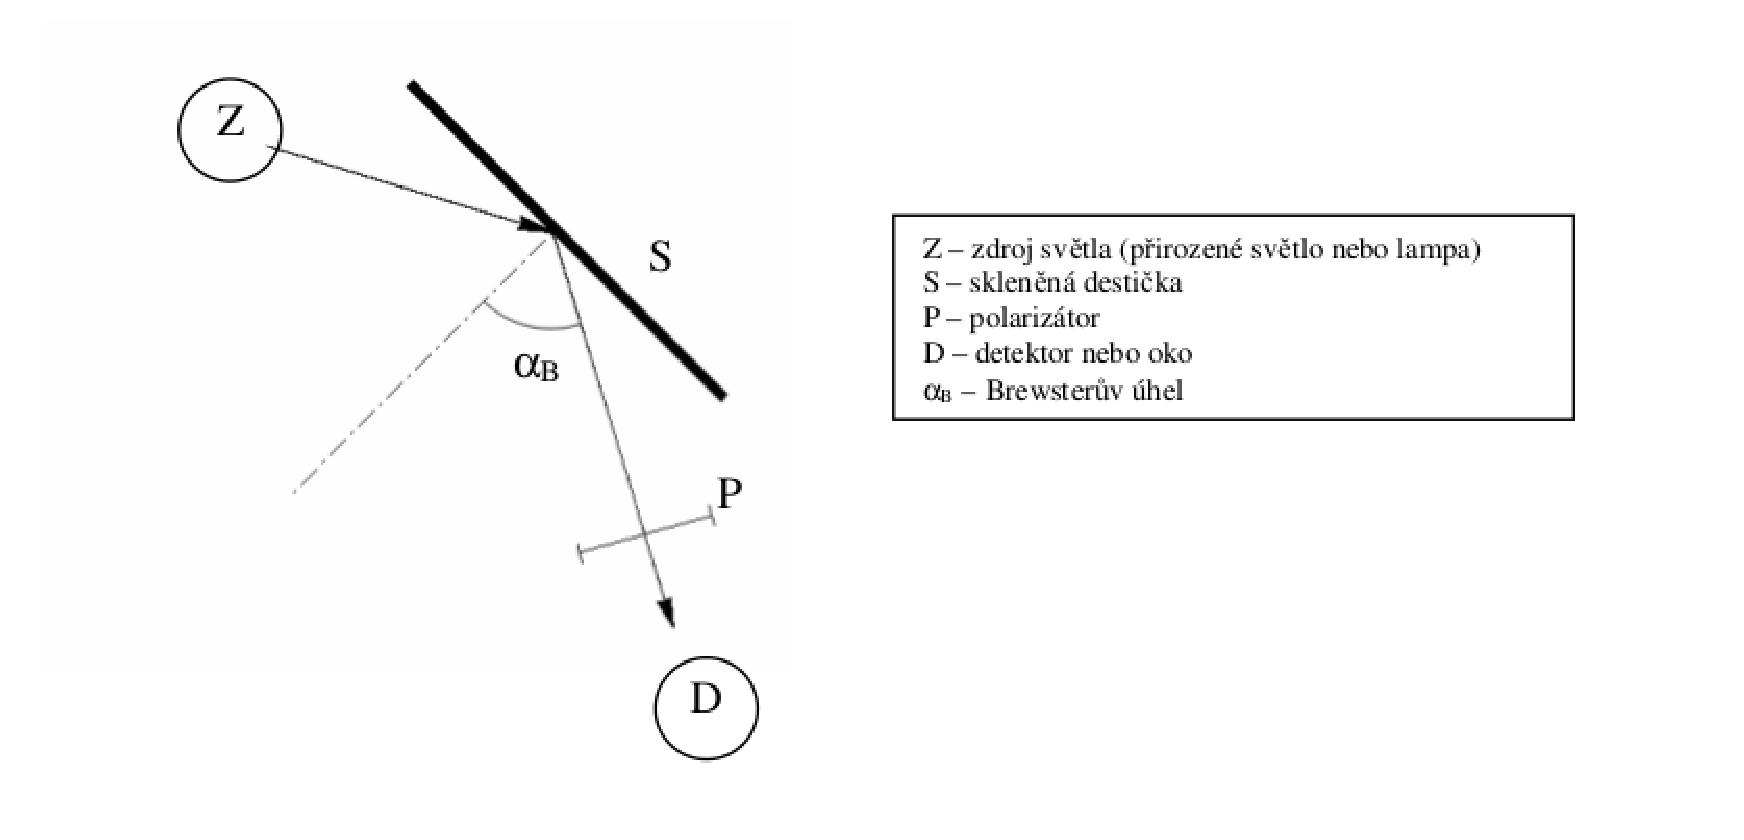
\includegraphics[width=6in]{obr1.eps}
\end{center}
\caption{Schéma pro polarizacu odrazem}
\label{Obr1}
\end{figure}

\begin{figure}
\begin{center}
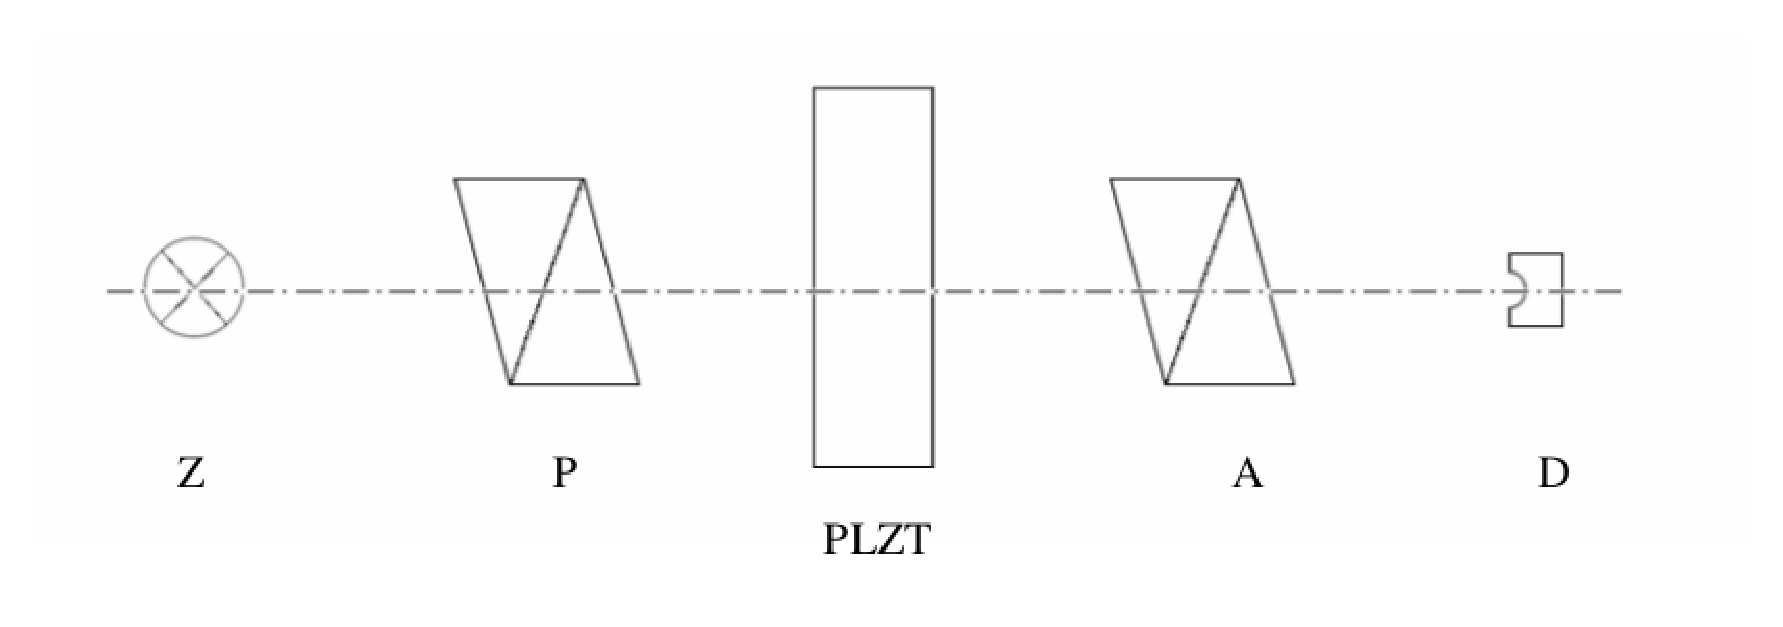
\includegraphics[width=6in]{obr2.eps}
\end{center}
\caption{Schéma aparatury pro měření Kerrova jevu}
\label{Obr2}
\end{figure}


\subsection{Aparatura}
Aparatura je sestavena dle \ref{Obr2}, přičemž za drojem světla je navíc umístěn přerušovač svazku, který byl po celou dobu měření otevřený. Za detektorem byl navíc 
umístěn fotonásobič, jehož výstupní hodnota po příslušném zesílení (dále značeno $Z$) byla odečítána na voltmetru ($U_{det}$). Relativní intenzita bude dále 
stanovena z této hodnoty dle vztahu
\begin{eqnarray}
I=Z_0U_{det}/Z,
\end{eqnarray}
kde $Z_0=100$, což byla hodnota zesílení použitá pro většinu měření. Použití jiného zesílení budé dále zdlrazněno. Její jednotka bude značena $\RJ$.
Chyba intenzity je určena z nejistoty voltmetru, která byla $\pm(0.2 \% + 3\mbox{d})$
Polarizátory byly umístěny do stojanů tak, aby odraz od přední strany dopadal do roviny paprsku kolmé na svislý směr polarizace. Odraz byl 
lehce pod zdorjem světla. Takto byla zajištěna kolmost polarizátoru. Vzorek PLZT byl umístěn ve vlastním držáku, ve kterém již byl natočen o úhel 45$\st$. 
Velikost vzorku byla menší než šířka laserového svazku.
Proto byl mezi dělič a polarizátor umístěn filt, který svazek zúžil. Přesto však byly znatelné odrazy od držáku vzorku.

\subsection{Intenzita na detektoru bez zdroje světla}
Vzhledem k tomum že úloha nebyla v zatemněné místnosti jsem nejprve určil hodnotu pro nulovou intenzitu ze zdroje světla. Bez zatemnění oken jsem přibližně v intervalu 
30 sekund naměřil hodnoty shrnuté v tabulce \ref{I0a}. V rámci měření jsem simuloval pohyb lidí po místnosti různým stíněním světla jdoucího především z okna.

\begin{table}
$$
\begin{array}{|c|c|c|c|c|c|c|c|c|c|c|}
\hline
I/\mbox{RJ}&   0.34&   0.34&   0.33&   0.34&   0.32&   0.33&   0.33&   0.34&   0.33&   0.34 \\ \hline
\end{array}
$$
\caption{Intenzita na detektoru bez zdroje světla.}
\label{I0a}
\end{table}

Z těchto hodnot jsem stanovil staistickou hodnotu pro nulovou intenzitu
\begin{eqnarray}
I_{00}=(0.33\pm0.03)\mbox{RJ}
\label{I00}
\end{eqnarray}

Stejné měření jsem také provedl při zatemnění místnosti. Za tmy byla nulová hodnota stabilně na hodnotě
\begin{eqnarray}
I_{t00}=(0.27\pm0.03)\mbox{RJ}
\label{It00}
\end{eqnarray}

\subsection{Svislost polarizace zdroje světla}
Při různých polohách polarizátoru a analyzátoru jsem za tmy měřil intenzity bez přítomnosti vzorku, abych určil, zda z laseru vychází pžedevším svisle polarizvané světlo. 
Hodnoty jsou shrnuty v tabulce \ref{TBV}, přičemž při nastavení obou filtrů na 0$\st$ byla hodnota na detektru mimo rozsah. Při měření jsem zároveň ověřoval účinnost 
zkřížení filtrů.

\begin{table}
$$
\begin{array}{|c|c|c|}
\hline
\mbox{P}/\st&   \mbox{A}/\st&   I/\RJ \\ \hline
-90&    0&  0.27 \\ \hline
0&  90& 0.27 \\ \hline
0&  -90&    0.28 \\ \hline
90& 90& 0.42 \\ \hline
90& 0&  0.27 \\ \hline
\end{array}
$$
\caption{Intenzity bez vzorku pro různé polohy polarizátoru (P) a analyzátoru (A).}
\label{TBV}
\end{table}

\subsection{Závislost intenzity prošlého světla na příčném napětí}
Nyní jsem zkřížil polarizační filtry a v závislosti na napětí mezi elektrodami vzorku ($U_{vz}$) jsem odečítal intenzitu na detektoru. Vzhledem k relaxační dobš vzorku 
jsem volil různé doby odečtení intenzity po nastavení napětí. Tato doba byla 30 respektive 60 sekund na zněnu napětí o 50 V, přičemž výsledky jsou v tabulkách \ref{TM30} reps \ref{TM60}. Nakonec vždyzměřím opět hodnotu pro nulové napětí, abych ověřil zda nedošlo k poškození vzorku nebo nějaké hrubé změně na aparatuře.

\begin{table}
$$
\begin{array}{|c|c|}
\hline
U_{vz}/\mbox{V}&    I/\RJ \\ \hline
0\pm 2&0.33\pm 0.03 \\ \hline
52\pm 2&0.34\pm 0.03 \\ \hline
104\pm 2&0.34\pm 0.03 \\ \hline
152\pm 2&0.34\pm 0.03 \\ \hline
207\pm 2&0.34\pm 0.03 \\ \hline
249\pm 2&0.34\pm 0.03 \\ \hline
300\pm 2&0.34\pm 0.03 \\ \hline
355\pm 2&0.34\pm 0.03 \\ \hline
406\pm 2&0.35\pm 0.03 \\ \hline
455\pm 2&0.37\pm 0.03 \\ \hline
509\pm 2&0.45\pm 0.03 \\ \hline
550\pm 2&0.58\pm 0.03 \\ \hline
609\pm 2&0.95\pm 0.03 \\ \hline
655\pm 2&1.50\pm 0.03 \\ \hline
703\pm 2&2.35\pm 0.03 \\ \hline
753\pm 2&3.36\pm 0.03 \\ \hline
803\pm 2&4.14\pm 0.03 \\ \hline
854\pm 2&4.05\pm 0.03 \\ \hline
902\pm 2&2.84\pm 0.03 \\ \hline
950\pm 2&1.08\pm 0.03 \\ \hline
995\pm 2&0.35\pm 0.03 \\ \hline
0\pm 2&0.34\pm 0.03 \\ \hline
\end{array}
$$
\caption{Intenzita na detektoru v závislosti na napětí na vzorku při relaxační době 30 s/50 V.}
\label{TM30}
\end{table}

\begin{table}
$$
\begin{array}{|c|c|}
\hline
U_{vz}/\mbox{V}&	I/\RJ \\ \hline
0\pm 2&0.35\pm 0.03 \\ \hline 
102\pm 2&0.35\pm 0.03 \\ \hline 
204\pm 2&0.35\pm 0.03 \\ \hline 
304\pm 2&0.34\pm 0.03 \\ \hline 
400\pm 2&0.35\pm 0.03 \\ \hline 
450\pm 2&0.37\pm 0.03 \\ \hline 
503\pm 2&0.45\pm 0.03 \\ \hline 
555\pm 2&0.63\pm 0.03 \\ \hline 
603\pm 2&0.98\pm 0.03 \\ \hline 
654\pm 2&1.57\pm 0.03 \\ \hline 
700\pm 2&2.54\pm 0.03 \\ \hline 
725\pm 2&2.94\pm 0.03 \\ \hline 
755\pm 2&7.63\pm 0.03 \\ \hline 
777\pm 2&4.06\pm 0.03 \\ \hline 
806\pm 2&4.48\pm 0.03 \\ \hline 
825\pm 2&4.60\pm 0.03 \\ \hline 
855\pm 2&4.52\pm 0.03 \\ \hline 
874\pm 2&4.20\pm 0.03 \\ \hline 
904\pm 2&3.41\pm 0.03 \\ \hline 
924\pm 2&2.71\pm 0.03 \\ \hline
952\pm 2&1.75\pm 0.03 \\ \hline 
973\pm 2&0.99\pm 0.03 \\ \hline 
1001\pm 2&0.46\pm 0.03 \\ \hline 
\end{array}
$$
\caption{Intenzita na detektoru v závislosti na napětí na vzorku při relaxační době 60 s/50 V.}
\label{TM60}
\end{table}

\subsection{Kerrova konstanta}
Na naměřené hodnoty jsem se pokusil nafitovat závislost uvedenou v rovnici \ref{I}. Tutokřivku jsem posunul o $I_{00}$. Dále jsem vzal v potaz, že 
hodnoty do 500 V neodpovídají teoretické závislosti. Ani při této korekci se programu gnuplot nepodařilo nafitovat odpovídající křivku. Nakonec jsem zkusil, 
že se vzorek při nízkých napětích vůbec nechová dle teorie a celou závislost jsem posunul doprava. Tak vznikly křivky na obrázcích \ref{G30} a \ref{G60}. 
Výsledné křivky mají předpisy
\begin{eqnarray}
I(U)&=&(4.00\pm0.06)\sin^2\left((U-(400\pm7))^2\frac{\pi (4.5\pm0.1)\cdot 10^{-9} 1.4\cdot 10^{-6}}{(1.5\cdot10^{-3})^2} \right)-0.335 \\
I(U)&=&(4.30\pm0.02)\sin^2\left((U-(390\pm3))^2\frac{\pi (4.12\pm0.06)\cdot 10^{-9} 1.4\cdot 10^{-6}}{(1.5\cdot10^{-3})^2} \right)-0.335
\end{eqnarray}
Z nich se snadno odečte Kerrova konstanta
\begin{eqnarray}
K_{30}&=&(4.5\pm0.1)\cdot 10^{-9} \mbox{m}/\mbox{V}^2\\
K_{60}&=&(4.12\pm0.06)\cdot 10^{-9} \mbox{m}/\mbox{V}^2
\end{eqnarray}

\begin{figure}
\begin{center}
% GNUPLOT: LaTeX picture with Postscript
\begingroup
  \makeatletter
  \providecommand\color[2][]{%
    \GenericError{(gnuplot) \space\space\space\@spaces}{%
      Package color not loaded in conjunction with
      terminal option `colourtext'%
    }{See the gnuplot documentation for explanation.%
    }{Either use 'blacktext' in gnuplot or load the package
      color.sty in LaTeX.}%
    \renewcommand\color[2][]{}%
  }%
  \providecommand\includegraphics[2][]{%
    \GenericError{(gnuplot) \space\space\space\@spaces}{%
      Package graphicx or graphics not loaded%
    }{See the gnuplot documentation for explanation.%
    }{The gnuplot epslatex terminal needs graphicx.sty or graphics.sty.}%
    \renewcommand\includegraphics[2][]{}%
  }%
  \providecommand\rotatebox[2]{#2}%
  \@ifundefined{ifGPcolor}{%
    \newif\ifGPcolor
    \GPcolorfalse
  }{}%
  \@ifundefined{ifGPblacktext}{%
    \newif\ifGPblacktext
    \GPblacktexttrue
  }{}%
  % define a \g@addto@macro without @ in the name:
  \let\gplgaddtomacro\g@addto@macro
  % define empty templates for all commands taking text:
  \gdef\gplbacktext{}%
  \gdef\gplfronttext{}%
  \makeatother
  \ifGPblacktext
    % no textcolor at all
    \def\colorrgb#1{}%
    \def\colorgray#1{}%
  \else
    % gray or color?
    \ifGPcolor
      \def\colorrgb#1{\color[rgb]{#1}}%
      \def\colorgray#1{\color[gray]{#1}}%
      \expandafter\def\csname LTw\endcsname{\color{white}}%
      \expandafter\def\csname LTb\endcsname{\color{black}}%
      \expandafter\def\csname LTa\endcsname{\color{black}}%
      \expandafter\def\csname LT0\endcsname{\color[rgb]{1,0,0}}%
      \expandafter\def\csname LT1\endcsname{\color[rgb]{0,1,0}}%
      \expandafter\def\csname LT2\endcsname{\color[rgb]{0,0,1}}%
      \expandafter\def\csname LT3\endcsname{\color[rgb]{1,0,1}}%
      \expandafter\def\csname LT4\endcsname{\color[rgb]{0,1,1}}%
      \expandafter\def\csname LT5\endcsname{\color[rgb]{1,1,0}}%
      \expandafter\def\csname LT6\endcsname{\color[rgb]{0,0,0}}%
      \expandafter\def\csname LT7\endcsname{\color[rgb]{1,0.3,0}}%
      \expandafter\def\csname LT8\endcsname{\color[rgb]{0.5,0.5,0.5}}%
    \else
      % gray
      \def\colorrgb#1{\color{black}}%
      \def\colorgray#1{\color[gray]{#1}}%
      \expandafter\def\csname LTw\endcsname{\color{white}}%
      \expandafter\def\csname LTb\endcsname{\color{black}}%
      \expandafter\def\csname LTa\endcsname{\color{black}}%
      \expandafter\def\csname LT0\endcsname{\color{black}}%
      \expandafter\def\csname LT1\endcsname{\color{black}}%
      \expandafter\def\csname LT2\endcsname{\color{black}}%
      \expandafter\def\csname LT3\endcsname{\color{black}}%
      \expandafter\def\csname LT4\endcsname{\color{black}}%
      \expandafter\def\csname LT5\endcsname{\color{black}}%
      \expandafter\def\csname LT6\endcsname{\color{black}}%
      \expandafter\def\csname LT7\endcsname{\color{black}}%
      \expandafter\def\csname LT8\endcsname{\color{black}}%
    \fi
  \fi
  \setlength{\unitlength}{0.0500bp}%
  \begin{picture}(7200.00,5040.00)%
    \gplgaddtomacro\gplbacktext{%
      \csname LTb\endcsname%
      \put(946,704){\makebox(0,0)[r]{\strut{} 0}}%
      \put(946,1213){\makebox(0,0)[r]{\strut{} 0.5}}%
      \put(946,1722){\makebox(0,0)[r]{\strut{} 1}}%
      \put(946,2231){\makebox(0,0)[r]{\strut{} 1.5}}%
      \put(946,2740){\makebox(0,0)[r]{\strut{} 2}}%
      \put(946,3248){\makebox(0,0)[r]{\strut{} 2.5}}%
      \put(946,3757){\makebox(0,0)[r]{\strut{} 3}}%
      \put(946,4266){\makebox(0,0)[r]{\strut{} 3.5}}%
      \put(946,4775){\makebox(0,0)[r]{\strut{} 4}}%
      \put(1078,484){\makebox(0,0){\strut{} 0}}%
      \put(1650,484){\makebox(0,0){\strut{} 100}}%
      \put(2223,484){\makebox(0,0){\strut{} 200}}%
      \put(2795,484){\makebox(0,0){\strut{} 300}}%
      \put(3368,484){\makebox(0,0){\strut{} 400}}%
      \put(3940,484){\makebox(0,0){\strut{} 500}}%
      \put(4513,484){\makebox(0,0){\strut{} 600}}%
      \put(5085,484){\makebox(0,0){\strut{} 700}}%
      \put(5658,484){\makebox(0,0){\strut{} 800}}%
      \put(6230,484){\makebox(0,0){\strut{} 900}}%
      \put(6803,484){\makebox(0,0){\strut{} 1000}}%
      \put(176,2739){\rotatebox{-270}{\makebox(0,0){\strut{}$I/\RJ$}}}%
      \put(3940,154){\makebox(0,0){\strut{}$U/\mbox{V}$}}%
    }%
    \gplgaddtomacro\gplfronttext{%
      \csname LTb\endcsname%
      \put(3718,4602){\makebox(0,0)[r]{\strut{}naměřené hodnoty}}%
      \csname LTb\endcsname%
      \put(3718,4382){\makebox(0,0)[r]{\strut{}fitovaná křivka}}%
    }%
    \gplbacktext
    \put(0,0){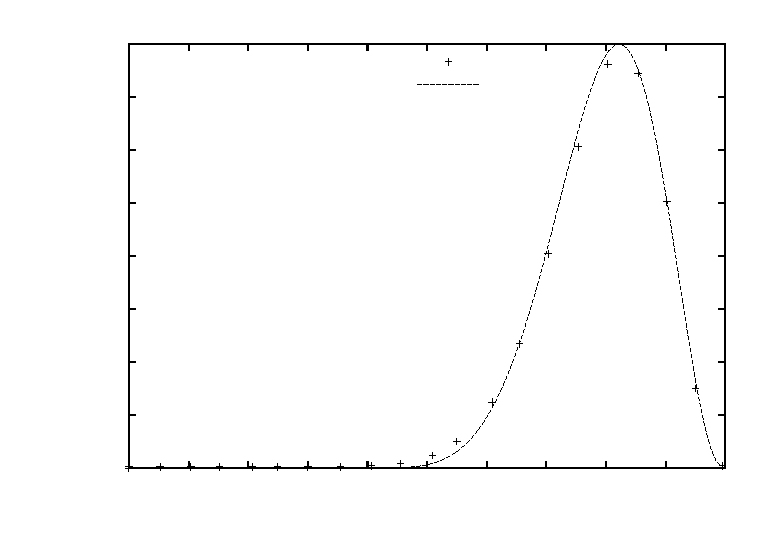
\includegraphics{G30}}%
    \gplfronttext
  \end{picture}%
\endgroup

\end{center}
\caption{Graf závislosti intenzity na napětí pro relaxační dobu 30 s.}
\label{G30}
\end{figure}

\begin{figure}
\begin{center}
% GNUPLOT: LaTeX picture with Postscript
\begingroup
  \makeatletter
  \providecommand\color[2][]{%
    \GenericError{(gnuplot) \space\space\space\@spaces}{%
      Package color not loaded in conjunction with
      terminal option `colourtext'%
    }{See the gnuplot documentation for explanation.%
    }{Either use 'blacktext' in gnuplot or load the package
      color.sty in LaTeX.}%
    \renewcommand\color[2][]{}%
  }%
  \providecommand\includegraphics[2][]{%
    \GenericError{(gnuplot) \space\space\space\@spaces}{%
      Package graphicx or graphics not loaded%
    }{See the gnuplot documentation for explanation.%
    }{The gnuplot epslatex terminal needs graphicx.sty or graphics.sty.}%
    \renewcommand\includegraphics[2][]{}%
  }%
  \providecommand\rotatebox[2]{#2}%
  \@ifundefined{ifGPcolor}{%
    \newif\ifGPcolor
    \GPcolorfalse
  }{}%
  \@ifundefined{ifGPblacktext}{%
    \newif\ifGPblacktext
    \GPblacktexttrue
  }{}%
  % define a \g@addto@macro without @ in the name:
  \let\gplgaddtomacro\g@addto@macro
  % define empty templates for all commands taking text:
  \gdef\gplbacktext{}%
  \gdef\gplfronttext{}%
  \makeatother
  \ifGPblacktext
    % no textcolor at all
    \def\colorrgb#1{}%
    \def\colorgray#1{}%
  \else
    % gray or color?
    \ifGPcolor
      \def\colorrgb#1{\color[rgb]{#1}}%
      \def\colorgray#1{\color[gray]{#1}}%
      \expandafter\def\csname LTw\endcsname{\color{white}}%
      \expandafter\def\csname LTb\endcsname{\color{black}}%
      \expandafter\def\csname LTa\endcsname{\color{black}}%
      \expandafter\def\csname LT0\endcsname{\color[rgb]{1,0,0}}%
      \expandafter\def\csname LT1\endcsname{\color[rgb]{0,1,0}}%
      \expandafter\def\csname LT2\endcsname{\color[rgb]{0,0,1}}%
      \expandafter\def\csname LT3\endcsname{\color[rgb]{1,0,1}}%
      \expandafter\def\csname LT4\endcsname{\color[rgb]{0,1,1}}%
      \expandafter\def\csname LT5\endcsname{\color[rgb]{1,1,0}}%
      \expandafter\def\csname LT6\endcsname{\color[rgb]{0,0,0}}%
      \expandafter\def\csname LT7\endcsname{\color[rgb]{1,0.3,0}}%
      \expandafter\def\csname LT8\endcsname{\color[rgb]{0.5,0.5,0.5}}%
    \else
      % gray
      \def\colorrgb#1{\color{black}}%
      \def\colorgray#1{\color[gray]{#1}}%
      \expandafter\def\csname LTw\endcsname{\color{white}}%
      \expandafter\def\csname LTb\endcsname{\color{black}}%
      \expandafter\def\csname LTa\endcsname{\color{black}}%
      \expandafter\def\csname LT0\endcsname{\color{black}}%
      \expandafter\def\csname LT1\endcsname{\color{black}}%
      \expandafter\def\csname LT2\endcsname{\color{black}}%
      \expandafter\def\csname LT3\endcsname{\color{black}}%
      \expandafter\def\csname LT4\endcsname{\color{black}}%
      \expandafter\def\csname LT5\endcsname{\color{black}}%
      \expandafter\def\csname LT6\endcsname{\color{black}}%
      \expandafter\def\csname LT7\endcsname{\color{black}}%
      \expandafter\def\csname LT8\endcsname{\color{black}}%
    \fi
  \fi
  \setlength{\unitlength}{0.0500bp}%
  \begin{picture}(7200.00,5040.00)%
    \gplgaddtomacro\gplbacktext{%
      \csname LTb\endcsname%
      \put(946,704){\makebox(0,0)[r]{\strut{} 0}}%
      \put(946,1156){\makebox(0,0)[r]{\strut{} 0.5}}%
      \put(946,1609){\makebox(0,0)[r]{\strut{} 1}}%
      \put(946,2061){\makebox(0,0)[r]{\strut{} 1.5}}%
      \put(946,2513){\makebox(0,0)[r]{\strut{} 2}}%
      \put(946,2966){\makebox(0,0)[r]{\strut{} 2.5}}%
      \put(946,3418){\makebox(0,0)[r]{\strut{} 3}}%
      \put(946,3870){\makebox(0,0)[r]{\strut{} 3.5}}%
      \put(946,4323){\makebox(0,0)[r]{\strut{} 4}}%
      \put(946,4775){\makebox(0,0)[r]{\strut{} 4.5}}%
      \put(1078,484){\makebox(0,0){\strut{} 0}}%
      \put(2217,484){\makebox(0,0){\strut{} 200}}%
      \put(3357,484){\makebox(0,0){\strut{} 400}}%
      \put(4496,484){\makebox(0,0){\strut{} 600}}%
      \put(5635,484){\makebox(0,0){\strut{} 800}}%
      \put(6775,484){\makebox(0,0){\strut{} 1000}}%
      \put(176,2739){\rotatebox{-270}{\makebox(0,0){\strut{}$I/\RJ$}}}%
      \put(3940,154){\makebox(0,0){\strut{}$U/\mbox{V}$}}%
    }%
    \gplgaddtomacro\gplfronttext{%
      \csname LTb\endcsname%
      \put(3718,4602){\makebox(0,0)[r]{\strut{}naměřené hodnoty}}%
      \csname LTb\endcsname%
      \put(3718,4382){\makebox(0,0)[r]{\strut{}fitovaná křivka}}%
    }%
    \gplbacktext
    \put(0,0){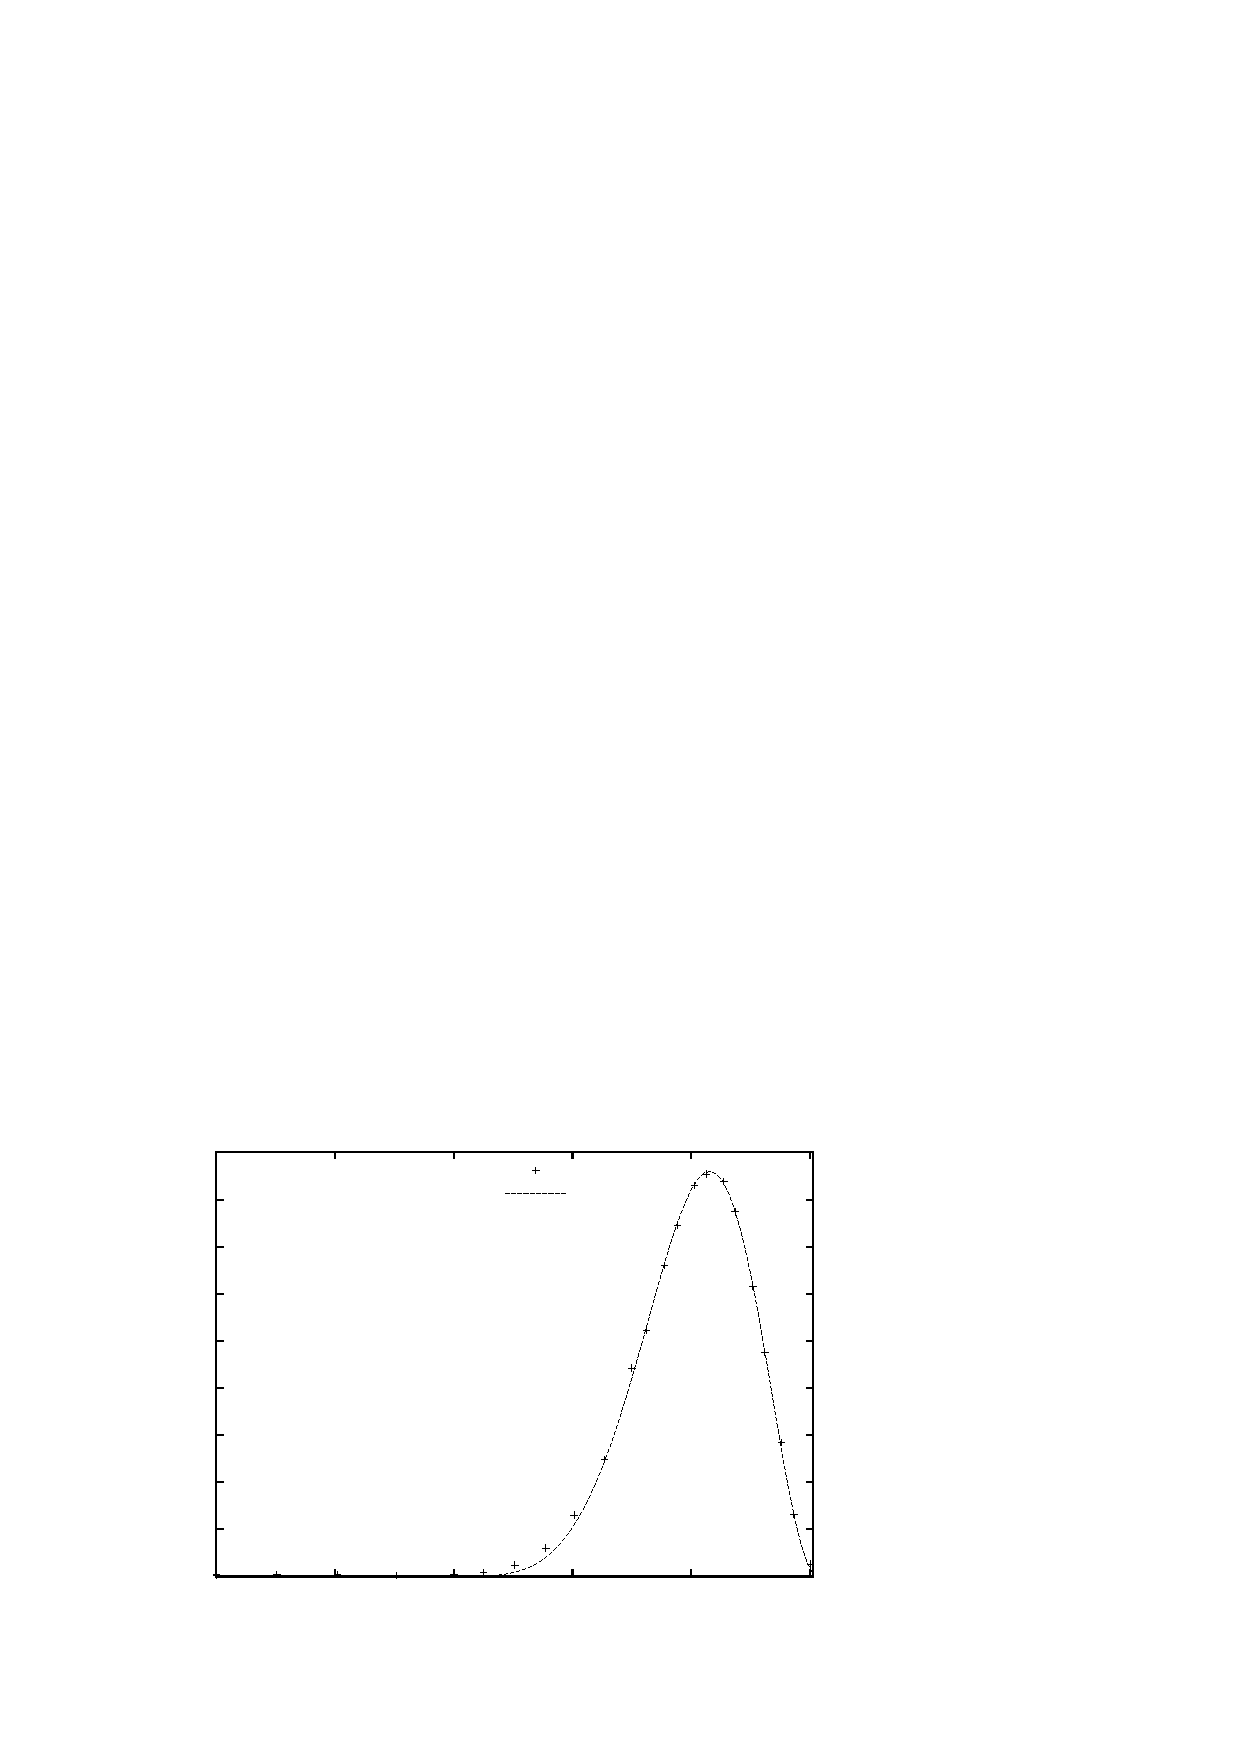
\includegraphics{G60}}%
    \gplfronttext
  \end{picture}%
\endgroup

\end{center}
\caption{Graf závislosti intenzity na napětí pro relaxační dobu 60 s.}
\label{G60}
\end{figure}

Jako druhou metou pro zjištění Kerrovy konstanty jsem použil vynesení čtverce napětí na fázovém posunutí. Obrázky \ref{G30b} a \ref{G60b}. Kerrova konstanta se dá zle vzorce \ref{Kb} dopočítat ze směrnice 
této závislosti. Při fitování křivky na tyto hodnoty jsem opět počítal s tím, že vzorek na nízká napětí nereagoval a proto se nechoval dle teoretické závislosti. 
Z fitu lze vičíst, že toto napětí se pohybovalo až kolem hodnoty 550 V. Nafitované křivky pro první respektive druhé měření naleznete pod rovnicemi \ref{f1} resp \ref{f2}. 
Dopočítaná Kerrova konstanta je rovnice \ref{K30b} resp \ref{K60b}.
\begin{eqnarray}
\label{f1}
U^2(\Delta)&=&(104500\pm 2700)\Delta+(345000\pm 11000) \mbox{V}^2 \\
\label{K30b}
K_{30b}&=&(4.0\pm0.1)\cdot 10^{-9}\mbox{m}/\mbox{V}^2 \\
\label{f2}
U^2(\Delta)&=&(113900\pm 1900)\Delta+(329000\pm 7000) \mbox{V}^2 \\
\label{K60b}
K_{60b}&=&(3.65\pm0.06)\cdot 10^{-9}\mbox{m}/\mbox{V}^2 
\end{eqnarray}

Pokud rovnici \ref{f2} odmocníme a dosadíme fázový posun $\Delta=2\pi$, získáme hodnotu půlvlnného napětí. Tato hodnota je
\begin{eqnarray}
U_{\lambda/2}=1020\pm 20 \mbox{V}
\end{eqnarray}

\begin{figure}
\begin{center}
% GNUPLOT: LaTeX picture with Postscript
\begingroup
  \makeatletter
  \providecommand\color[2][]{%
    \GenericError{(gnuplot) \space\space\space\@spaces}{%
      Package color not loaded in conjunction with
      terminal option `colourtext'%
    }{See the gnuplot documentation for explanation.%
    }{Either use 'blacktext' in gnuplot or load the package
      color.sty in LaTeX.}%
    \renewcommand\color[2][]{}%
  }%
  \providecommand\includegraphics[2][]{%
    \GenericError{(gnuplot) \space\space\space\@spaces}{%
      Package graphicx or graphics not loaded%
    }{See the gnuplot documentation for explanation.%
    }{The gnuplot epslatex terminal needs graphicx.sty or graphics.sty.}%
    \renewcommand\includegraphics[2][]{}%
  }%
  \providecommand\rotatebox[2]{#2}%
  \@ifundefined{ifGPcolor}{%
    \newif\ifGPcolor
    \GPcolorfalse
  }{}%
  \@ifundefined{ifGPblacktext}{%
    \newif\ifGPblacktext
    \GPblacktexttrue
  }{}%
  % define a \g@addto@macro without @ in the name:
  \let\gplgaddtomacro\g@addto@macro
  % define empty templates for all commands taking text:
  \gdef\gplbacktext{}%
  \gdef\gplfronttext{}%
  \makeatother
  \ifGPblacktext
    % no textcolor at all
    \def\colorrgb#1{}%
    \def\colorgray#1{}%
  \else
    % gray or color?
    \ifGPcolor
      \def\colorrgb#1{\color[rgb]{#1}}%
      \def\colorgray#1{\color[gray]{#1}}%
      \expandafter\def\csname LTw\endcsname{\color{white}}%
      \expandafter\def\csname LTb\endcsname{\color{black}}%
      \expandafter\def\csname LTa\endcsname{\color{black}}%
      \expandafter\def\csname LT0\endcsname{\color[rgb]{1,0,0}}%
      \expandafter\def\csname LT1\endcsname{\color[rgb]{0,1,0}}%
      \expandafter\def\csname LT2\endcsname{\color[rgb]{0,0,1}}%
      \expandafter\def\csname LT3\endcsname{\color[rgb]{1,0,1}}%
      \expandafter\def\csname LT4\endcsname{\color[rgb]{0,1,1}}%
      \expandafter\def\csname LT5\endcsname{\color[rgb]{1,1,0}}%
      \expandafter\def\csname LT6\endcsname{\color[rgb]{0,0,0}}%
      \expandafter\def\csname LT7\endcsname{\color[rgb]{1,0.3,0}}%
      \expandafter\def\csname LT8\endcsname{\color[rgb]{0.5,0.5,0.5}}%
    \else
      % gray
      \def\colorrgb#1{\color{black}}%
      \def\colorgray#1{\color[gray]{#1}}%
      \expandafter\def\csname LTw\endcsname{\color{white}}%
      \expandafter\def\csname LTb\endcsname{\color{black}}%
      \expandafter\def\csname LTa\endcsname{\color{black}}%
      \expandafter\def\csname LT0\endcsname{\color{black}}%
      \expandafter\def\csname LT1\endcsname{\color{black}}%
      \expandafter\def\csname LT2\endcsname{\color{black}}%
      \expandafter\def\csname LT3\endcsname{\color{black}}%
      \expandafter\def\csname LT4\endcsname{\color{black}}%
      \expandafter\def\csname LT5\endcsname{\color{black}}%
      \expandafter\def\csname LT6\endcsname{\color{black}}%
      \expandafter\def\csname LT7\endcsname{\color{black}}%
      \expandafter\def\csname LT8\endcsname{\color{black}}%
    \fi
  \fi
  \setlength{\unitlength}{0.0500bp}%
  \begin{picture}(7200.00,5040.00)%
    \gplgaddtomacro\gplbacktext{%
      \csname LTb\endcsname%
      \put(1342,898){\makebox(0,0)[r]{\strut{} 200000}}%
      \put(1342,1383){\makebox(0,0)[r]{\strut{} 300000}}%
      \put(1342,1867){\makebox(0,0)[r]{\strut{} 400000}}%
      \put(1342,2352){\makebox(0,0)[r]{\strut{} 500000}}%
      \put(1342,2836){\makebox(0,0)[r]{\strut{} 600000}}%
      \put(1342,3321){\makebox(0,0)[r]{\strut{} 700000}}%
      \put(1342,3806){\makebox(0,0)[r]{\strut{} 800000}}%
      \put(1342,4290){\makebox(0,0)[r]{\strut{} 900000}}%
      \put(1342,4775){\makebox(0,0)[r]{\strut{} 1e+06}}%
      \put(2169,484){\makebox(0,0){\strut{} 1}}%
      \put(2941,484){\makebox(0,0){\strut{} 2}}%
      \put(3714,484){\makebox(0,0){\strut{} 3}}%
      \put(4486,484){\makebox(0,0){\strut{} 4}}%
      \put(5258,484){\makebox(0,0){\strut{} 5}}%
      \put(6031,484){\makebox(0,0){\strut{} 6}}%
      \put(6803,484){\makebox(0,0){\strut{} 7}}%
      \put(176,2739){\rotatebox{-270}{\makebox(0,0){\strut{}$(U/\mbox{V})^2$}}}%
      \put(4138,154){\makebox(0,0){\strut{}$\Delta/\mbox{rad}$}}%
    }%
    \gplgaddtomacro\gplfronttext{%
      \csname LTb\endcsname%
      \put(4114,4602){\makebox(0,0)[r]{\strut{}naměřené hodnoty}}%
      \csname LTb\endcsname%
      \put(4114,4382){\makebox(0,0)[r]{\strut{}fitovaná křivka}}%
    }%
    \gplbacktext
    \put(0,0){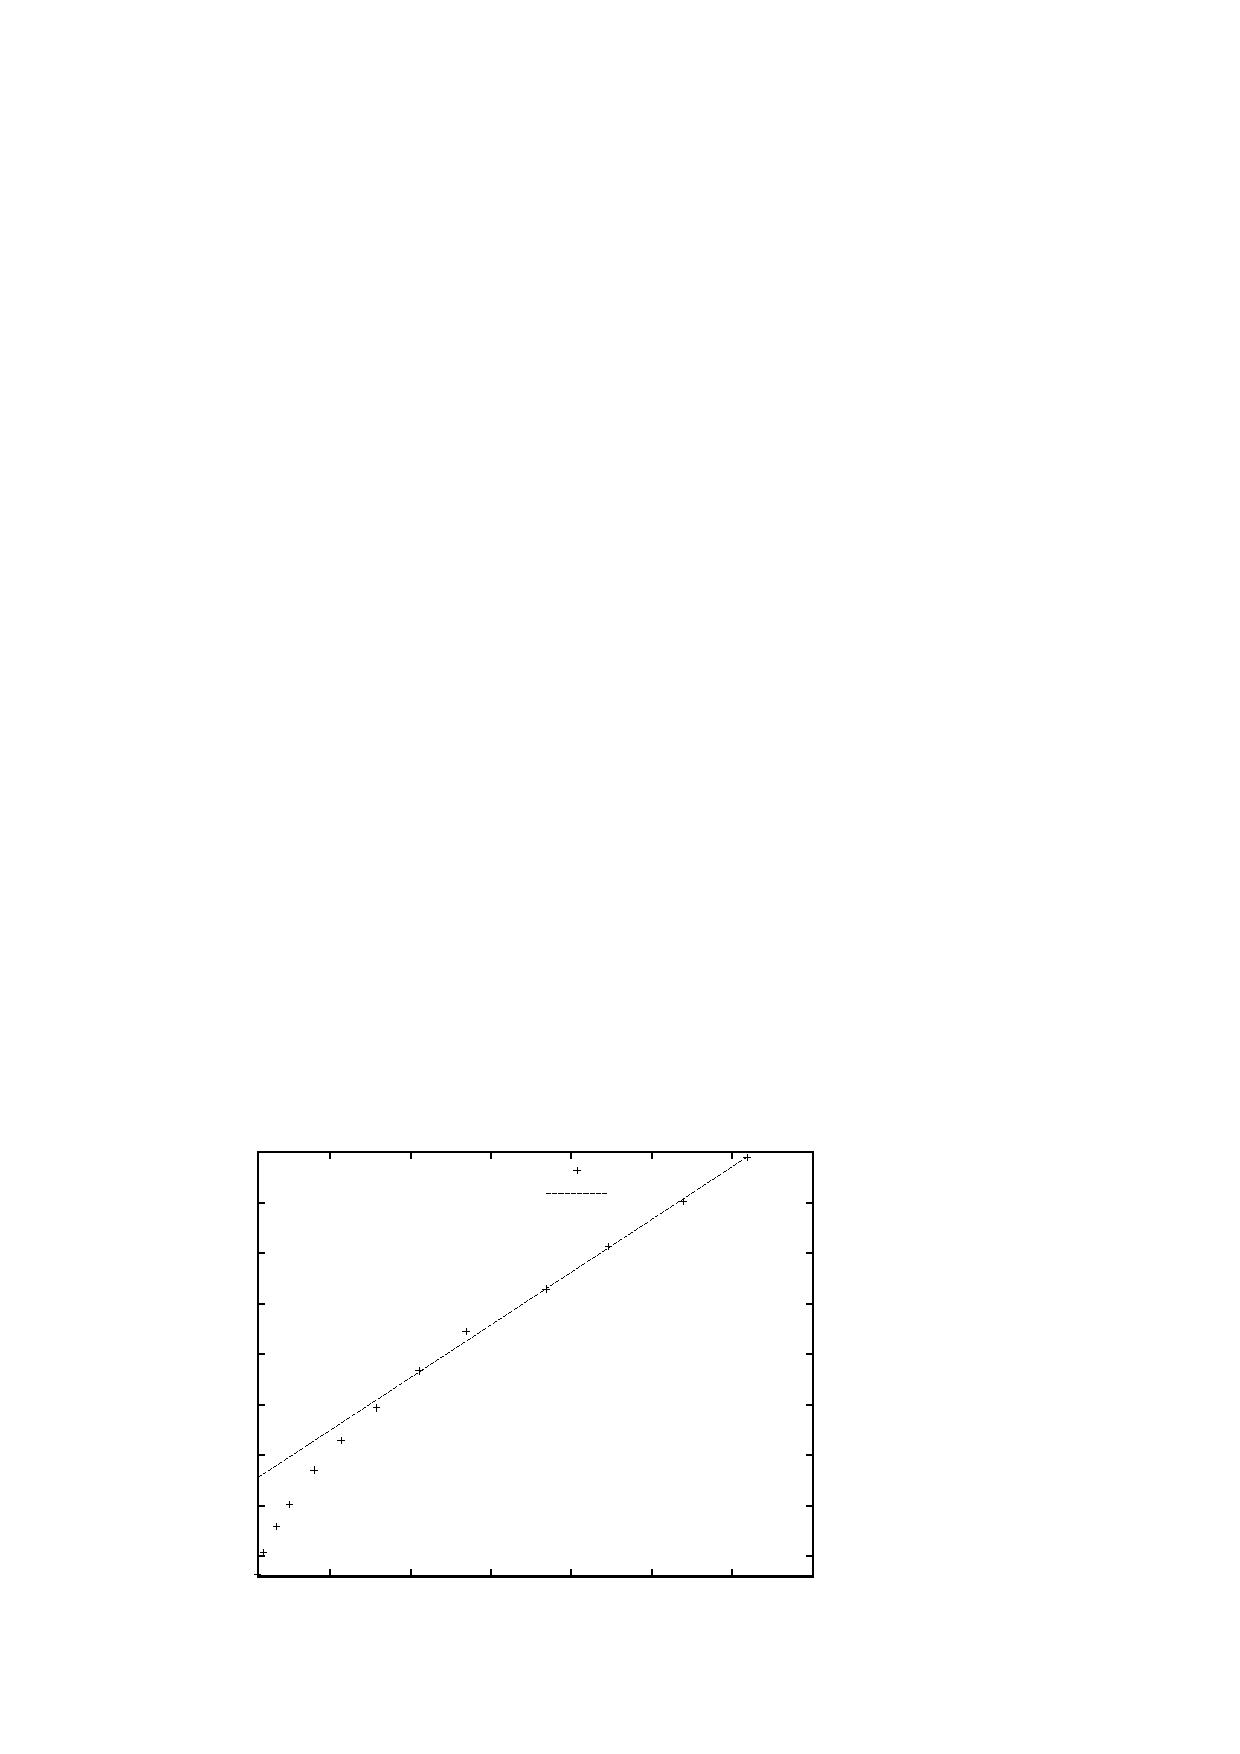
\includegraphics{G30b}}%
    \gplfronttext
  \end{picture}%
\endgroup

\end{center}
\caption{Graf závislosti čtverce napětí na posunutí fáze pro relaxační dobu 30 s.}
\label{G30b}
\end{figure}

\begin{figure}
\begin{center}
% GNUPLOT: LaTeX picture with Postscript
\begingroup
  \makeatletter
  \providecommand\color[2][]{%
    \GenericError{(gnuplot) \space\space\space\@spaces}{%
      Package color not loaded in conjunction with
      terminal option `colourtext'%
    }{See the gnuplot documentation for explanation.%
    }{Either use 'blacktext' in gnuplot or load the package
      color.sty in LaTeX.}%
    \renewcommand\color[2][]{}%
  }%
  \providecommand\includegraphics[2][]{%
    \GenericError{(gnuplot) \space\space\space\@spaces}{%
      Package graphicx or graphics not loaded%
    }{See the gnuplot documentation for explanation.%
    }{The gnuplot epslatex terminal needs graphicx.sty or graphics.sty.}%
    \renewcommand\includegraphics[2][]{}%
  }%
  \providecommand\rotatebox[2]{#2}%
  \@ifundefined{ifGPcolor}{%
    \newif\ifGPcolor
    \GPcolorfalse
  }{}%
  \@ifundefined{ifGPblacktext}{%
    \newif\ifGPblacktext
    \GPblacktexttrue
  }{}%
  % define a \g@addto@macro without @ in the name:
  \let\gplgaddtomacro\g@addto@macro
  % define empty templates for all commands taking text:
  \gdef\gplbacktext{}%
  \gdef\gplfronttext{}%
  \makeatother
  \ifGPblacktext
    % no textcolor at all
    \def\colorrgb#1{}%
    \def\colorgray#1{}%
  \else
    % gray or color?
    \ifGPcolor
      \def\colorrgb#1{\color[rgb]{#1}}%
      \def\colorgray#1{\color[gray]{#1}}%
      \expandafter\def\csname LTw\endcsname{\color{white}}%
      \expandafter\def\csname LTb\endcsname{\color{black}}%
      \expandafter\def\csname LTa\endcsname{\color{black}}%
      \expandafter\def\csname LT0\endcsname{\color[rgb]{1,0,0}}%
      \expandafter\def\csname LT1\endcsname{\color[rgb]{0,1,0}}%
      \expandafter\def\csname LT2\endcsname{\color[rgb]{0,0,1}}%
      \expandafter\def\csname LT3\endcsname{\color[rgb]{1,0,1}}%
      \expandafter\def\csname LT4\endcsname{\color[rgb]{0,1,1}}%
      \expandafter\def\csname LT5\endcsname{\color[rgb]{1,1,0}}%
      \expandafter\def\csname LT6\endcsname{\color[rgb]{0,0,0}}%
      \expandafter\def\csname LT7\endcsname{\color[rgb]{1,0.3,0}}%
      \expandafter\def\csname LT8\endcsname{\color[rgb]{0.5,0.5,0.5}}%
    \else
      % gray
      \def\colorrgb#1{\color{black}}%
      \def\colorgray#1{\color[gray]{#1}}%
      \expandafter\def\csname LTw\endcsname{\color{white}}%
      \expandafter\def\csname LTb\endcsname{\color{black}}%
      \expandafter\def\csname LTa\endcsname{\color{black}}%
      \expandafter\def\csname LT0\endcsname{\color{black}}%
      \expandafter\def\csname LT1\endcsname{\color{black}}%
      \expandafter\def\csname LT2\endcsname{\color{black}}%
      \expandafter\def\csname LT3\endcsname{\color{black}}%
      \expandafter\def\csname LT4\endcsname{\color{black}}%
      \expandafter\def\csname LT5\endcsname{\color{black}}%
      \expandafter\def\csname LT6\endcsname{\color{black}}%
      \expandafter\def\csname LT7\endcsname{\color{black}}%
      \expandafter\def\csname LT8\endcsname{\color{black}}%
    \fi
  \fi
  \setlength{\unitlength}{0.0500bp}%
  \begin{picture}(7200.00,5040.00)%
    \gplgaddtomacro\gplbacktext{%
      \csname LTb\endcsname%
      \put(1474,877){\makebox(0,0)[r]{\strut{} 200000}}%
      \put(1474,1310){\makebox(0,0)[r]{\strut{} 300000}}%
      \put(1474,1743){\makebox(0,0)[r]{\strut{} 400000}}%
      \put(1474,2176){\makebox(0,0)[r]{\strut{} 500000}}%
      \put(1474,2610){\makebox(0,0)[r]{\strut{} 600000}}%
      \put(1474,3043){\makebox(0,0)[r]{\strut{} 700000}}%
      \put(1474,3476){\makebox(0,0)[r]{\strut{} 800000}}%
      \put(1474,3909){\makebox(0,0)[r]{\strut{} 900000}}%
      \put(1474,4342){\makebox(0,0)[r]{\strut{} 1e+06}}%
      \put(1474,4775){\makebox(0,0)[r]{\strut{} 1.1e+06}}%
      \put(2399,484){\makebox(0,0){\strut{} 1}}%
      \put(3280,484){\makebox(0,0){\strut{} 2}}%
      \put(4160,484){\makebox(0,0){\strut{} 3}}%
      \put(5041,484){\makebox(0,0){\strut{} 4}}%
      \put(5922,484){\makebox(0,0){\strut{} 5}}%
      \put(6803,484){\makebox(0,0){\strut{} 6}}%
      \put(176,2739){\rotatebox{-270}{\makebox(0,0){\strut{}$(U/\mbox{V})^2$}}}%
      \put(4204,154){\makebox(0,0){\strut{}$\Delta/\mbox{rad}$}}%
    }%
    \gplgaddtomacro\gplfronttext{%
      \csname LTb\endcsname%
      \put(4246,4602){\makebox(0,0)[r]{\strut{}naměřené hodnoty}}%
      \csname LTb\endcsname%
      \put(4246,4382){\makebox(0,0)[r]{\strut{}fitovaná křivka}}%
    }%
    \gplbacktext
    \put(0,0){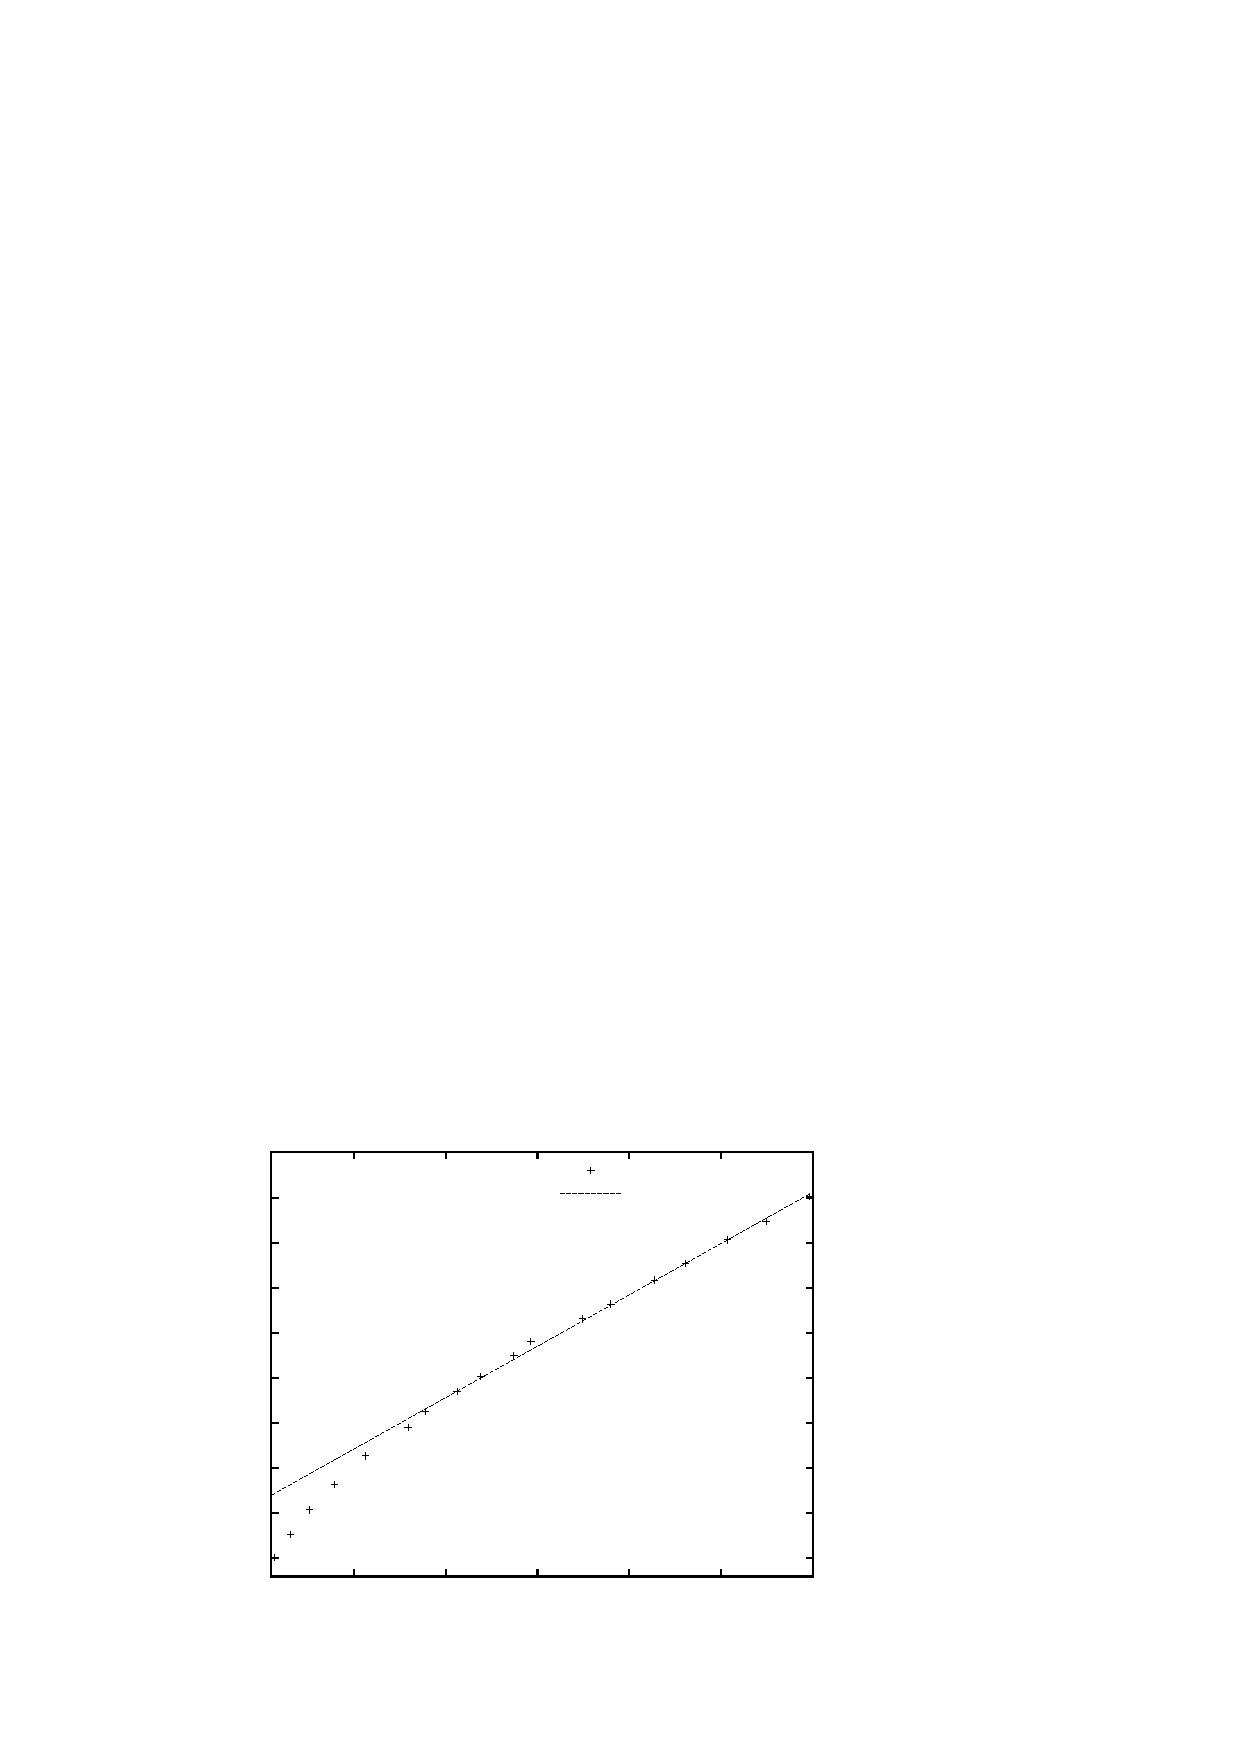
\includegraphics{G60b}}%
    \gplfronttext
  \end{picture}%
\endgroup

\end{center}
\caption{Graf závislosti čtverce napětí na posunutí fáze pro relaxační dobu 60 s.}
\label{G60b}
\end{figure}

Fázový posun jsem se také pokusil zjisti za pomoci změny nastavení analyzátoru. Pro jednotlivá napětí na elektrodách jsem vždy hledal minimum intenzity na detektoru. 
Fázový posun jsem získal posunem naměření hodnoty o $90\st$ a následným vynásobením dvěmi.
Výsledky jsem následně zpracoval stejným postupem jako v minulém případě. První měření bylo pouze orientační. Začal jsem až na hodnotě 300 V. Doba mezi odečítáním 
hodnot nebyla nijak určená a lišila se podle toho, jak śpěšně se mi dařilo neléz minimum. Chyba u polohy analyzátoru je odhadnuta ze šířky minima. Výsledky jsou v tabulce \ref{T5a}. Zpracovaný graf je na obrázku 
\ref{5a}. Dopočtená Kerrova konstanta stanovená z tohoto měření je
\begin{eqnarray}
K_{5a}=(3.6\pm 0.6) \cdot 10^{-9} \mV
\end{eqnarray}

\begin{table}
$$
\begin{array}{|c|c|}
\hline
U_{vz}\mbox{V}& A/\st \\ \hline
312 \pm 2 &   -90 \pm 4 \\ \hline
400 \pm 2 &   -90 \pm 4 \\ \hline
452 \pm 2 &   -90 \pm 4 \\ \hline
504 \pm 2 &   -90 \pm 4 \\ \hline
557 \pm 2 &   -90 \pm 4 \\ \hline
604 \pm 2 &   -90 \pm 4 \\ \hline
653 \pm 2 &   -68 \pm 4 \\ \hline
703 \pm 2 &   -28 \pm 4 \\ \hline
751 \pm 2 &   -5 \pm 4 \\ \hline
805 \pm 2 &   -2 \pm 4 \\ \hline
854 \pm 2 &   5 \pm 4 \\ \hline
906 \pm 2 &   6 \pm 4 \\ \hline
952 \pm 2 &   29 \pm 4 \\ \hline
970 \pm 2 &   79 \pm 4 \\ \hline
997 \pm 2 &   90 \pm 4 \\ \hline
\end{array}
$$
\caption{Polohy analyzátoru při minimální intenzitě na detektoru pro první měření.}
\label{T5a}
\end{table}

Další měření jsem prováděl o něco hustšeji. Také jsem se snažil držet pravidelnější interval mezi odečítáním hodnot. Pozice minim jsem navíc zpřesňoval použitím většího zesílení. Nemářené hodnoty jsou v tabulce \ref{T5b}, zpracovaný graf na obrázku \ref{5b} a dopočtená Kerrova konstanta je
\begin{eqnarray}
K_{5b}=(3.0\pm0.4) \cdot 10^{-9} \mV
\end{eqnarray}

\begin{table}
$$
\begin{array}{|c|c|c|c|c|}
\hline
&   \multicolumn{2}{c|}{Z=100}& \multicolumn{2}{c|}{Z=1000} \\ \hline
U_{vz}\mbox{V}& A/\st&  I/\RJ&  A/\st&  I/\RJ   \\ \hline
0 \pm 2 &   -90 \pm 4&  0.33\pm 0.03& &  \\ \hline
303 \pm 2 &   -90 \pm 4& 0.33 \pm 0.03& & \\ \hline
401 \pm 2 &   -90 \pm 4& 0.34 \pm 0.03& & \\ \hline
503 \pm 2 &   -90 \pm 4& 0.41 \pm 0.03& & \\ \hline
552 \pm 2 &   -90 \pm 4& 0.51 \pm 0.03& &  \\ \hline
599 \pm 2 &   -90 \pm 4& 0.75 \pm 0.03& -90 \pm 4 & 0.501 \pm 0.003 \\ \hline
650 \pm 2 &   -80 \pm 4& 1.28 \pm 0.03& -81 \pm 4& 1.002 \pm 0.003 \\ \hline
700 \pm 2 &   -69 \pm 4& 1.66 \pm 0.03& & \\ \hline
723 \pm 2 &   -28 \pm 4& 1.67\pm 0.03& &  \\ \hline
749 \pm 2 &   -19 \pm 4& 1.54\pm 0.03& &  \\ \hline
774 \pm 2 &   -13 \pm 4& 1.20\pm 0.03& -14\pm 2 & 0.900 \pm 0.003  \\ \hline
799 \pm 2 &   -3 \pm 4& 0.89\pm 0.03& -4\pm 2 & 0.605 \pm 0.003  \\ \hline
825 \pm 2 &   3 \pm 4& 0.60\pm 0.03& 5\pm 2 & 0.335 \pm 0.003  \\ \hline
850 \pm 2 &   7 \pm 4& 0.43\pm 0.03& 7\pm 2 & 0.162 \pm 0.003  \\ \hline
877 \pm 2 &   9 \pm 4& 0.37\pm 0.03& 7\pm 2 & 0.118 \pm 0.003  \\ \hline
902 \pm 2 &   8 \pm 4& 0.50\pm 0.03& 8\pm 2 & 0.293 \pm 0.003  \\ \hline
927 \pm 2 &   8 \pm 4& 0.77\pm 0.03& 9\pm 2 & 0.573 \pm 0.003  \\ \hline
953 \pm 2 &   13 \pm 4& 1.34\pm 0.03& &  \\ \hline
978 \pm 2 &   26 \pm 4& 1.89\pm 0.03& &  \\ \hline
1000 \pm 2 &   48 \pm 4& 1.95\pm 0.03& &  \\ \hline
\end{array}
$$
\caption{Polohy analyzátoru při minimální intenzitě na detektoru pro druhé měření.}
\label{T5b}
\end{table}

Poslední měření proběhlo při zatemněných oknech, abych vyloučil vliv 
okolního světla na výsledky. Při měření jsem si povšiml přítomnosti 
více minim. V tabulce \ref{T5c} jsou uvedena všechna. V grafu \ref{5c} pouza 
ta, která by měla odpovídat pozorovanému jevu. Dopočítaná Kerrova je
\begin{eqnarray}
K_{5c}=(3.1\pm0.4) \cdot 10^{-9} \mV
\end{eqnarray}

\begin{table}
$$
\begin{array}{|c|c|c|c|c|}
\hline
&   \multicolumn{2}{c|}{Z=100}& \multicolumn{2}{c|}{Z=1000} \\ \hline
U_{vz}\mbox{V}& A/\st&  I/\RJ&  A/\st&  I/\RJ   \\ \hline
0 \pm 2 &   -90 \pm 4&  0.28\pm 0.03& &  \\ \hline
454 \pm 2 &   -90 \pm 4& 0.39 \pm 0.03& & \\ \hline
503 \pm 2 &   -88 \pm 4& 0.45 \pm 0.03& & \\ \hline
550 \pm 2 &   -90 \pm 4& 0.59 \pm 0.03& -89 \pm 2 & 0.321 \pm 0.003  \\ \hline
600 \pm 2 &   -87 \pm 4& 0.80 \pm 0.03& -88 \pm 4 & 0.546 \pm 0.003 \\ \hline
654 \pm 2 &   -72 \pm 4|-86 \pm 4&1.50\pm0.03|1.25 \pm 0.03& -73 \pm 4& 1.220 \pm 0.003 \\ \hline
700 \pm 2 &   -47 \pm 4|-87 \pm 4&1.75\pm0.03|1.67 \pm 0.03& & \\ \hline
750 \pm 2 &   -38 \pm 4& 1.75\pm 0.03& &  \\ \hline
800 \pm 2 &   -16 \pm 4|-4 \pm 4& 1.02\pm0.03|0.95 \pm 0.03& & \\ \hline
856 \pm 2 &   -4 \pm 4& 0.47\pm0.03& -8\pm 2&0.195 \pm 0.003 \\ \hline
903 \pm 2 &   6 \pm 4& 0.34\pm0.03& 5\pm 2&0.102 \pm 0.003 \\ \hline
950 \pm 2 &   13 \pm 4& 0.76\pm0.03& 13\pm 2&0.642 \pm 0.003 \\ \hline
\end{array}
$$
\caption{Polohy analyzátoru při minimální intenzitě na detektoru pro třetí měření.}
\label{T5c}
\end{table}

\begin{figure}
\begin{center}
% GNUPLOT: LaTeX picture with Postscript
\begingroup
  \makeatletter
  \providecommand\color[2][]{%
    \GenericError{(gnuplot) \space\space\space\@spaces}{%
      Package color not loaded in conjunction with
      terminal option `colourtext'%
    }{See the gnuplot documentation for explanation.%
    }{Either use 'blacktext' in gnuplot or load the package
      color.sty in LaTeX.}%
    \renewcommand\color[2][]{}%
  }%
  \providecommand\includegraphics[2][]{%
    \GenericError{(gnuplot) \space\space\space\@spaces}{%
      Package graphicx or graphics not loaded%
    }{See the gnuplot documentation for explanation.%
    }{The gnuplot epslatex terminal needs graphicx.sty or graphics.sty.}%
    \renewcommand\includegraphics[2][]{}%
  }%
  \providecommand\rotatebox[2]{#2}%
  \@ifundefined{ifGPcolor}{%
    \newif\ifGPcolor
    \GPcolorfalse
  }{}%
  \@ifundefined{ifGPblacktext}{%
    \newif\ifGPblacktext
    \GPblacktexttrue
  }{}%
  % define a \g@addto@macro without @ in the name:
  \let\gplgaddtomacro\g@addto@macro
  % define empty templates for all commands taking text:
  \gdef\gplbacktext{}%
  \gdef\gplfronttext{}%
  \makeatother
  \ifGPblacktext
    % no textcolor at all
    \def\colorrgb#1{}%
    \def\colorgray#1{}%
  \else
    % gray or color?
    \ifGPcolor
      \def\colorrgb#1{\color[rgb]{#1}}%
      \def\colorgray#1{\color[gray]{#1}}%
      \expandafter\def\csname LTw\endcsname{\color{white}}%
      \expandafter\def\csname LTb\endcsname{\color{black}}%
      \expandafter\def\csname LTa\endcsname{\color{black}}%
      \expandafter\def\csname LT0\endcsname{\color[rgb]{1,0,0}}%
      \expandafter\def\csname LT1\endcsname{\color[rgb]{0,1,0}}%
      \expandafter\def\csname LT2\endcsname{\color[rgb]{0,0,1}}%
      \expandafter\def\csname LT3\endcsname{\color[rgb]{1,0,1}}%
      \expandafter\def\csname LT4\endcsname{\color[rgb]{0,1,1}}%
      \expandafter\def\csname LT5\endcsname{\color[rgb]{1,1,0}}%
      \expandafter\def\csname LT6\endcsname{\color[rgb]{0,0,0}}%
      \expandafter\def\csname LT7\endcsname{\color[rgb]{1,0.3,0}}%
      \expandafter\def\csname LT8\endcsname{\color[rgb]{0.5,0.5,0.5}}%
    \else
      % gray
      \def\colorrgb#1{\color{black}}%
      \def\colorgray#1{\color[gray]{#1}}%
      \expandafter\def\csname LTw\endcsname{\color{white}}%
      \expandafter\def\csname LTb\endcsname{\color{black}}%
      \expandafter\def\csname LTa\endcsname{\color{black}}%
      \expandafter\def\csname LT0\endcsname{\color{black}}%
      \expandafter\def\csname LT1\endcsname{\color{black}}%
      \expandafter\def\csname LT2\endcsname{\color{black}}%
      \expandafter\def\csname LT3\endcsname{\color{black}}%
      \expandafter\def\csname LT4\endcsname{\color{black}}%
      \expandafter\def\csname LT5\endcsname{\color{black}}%
      \expandafter\def\csname LT6\endcsname{\color{black}}%
      \expandafter\def\csname LT7\endcsname{\color{black}}%
      \expandafter\def\csname LT8\endcsname{\color{black}}%
    \fi
  \fi
  \setlength{\unitlength}{0.0500bp}%
  \begin{picture}(7200.00,5040.00)%
    \gplgaddtomacro\gplbacktext{%
      \csname LTb\endcsname%
      \put(1474,704){\makebox(0,0)[r]{\strut{} 200000}}%
      \put(1474,1156){\makebox(0,0)[r]{\strut{} 300000}}%
      \put(1474,1609){\makebox(0,0)[r]{\strut{} 400000}}%
      \put(1474,2061){\makebox(0,0)[r]{\strut{} 500000}}%
      \put(1474,2513){\makebox(0,0)[r]{\strut{} 600000}}%
      \put(1474,2966){\makebox(0,0)[r]{\strut{} 700000}}%
      \put(1474,3418){\makebox(0,0)[r]{\strut{} 800000}}%
      \put(1474,3870){\makebox(0,0)[r]{\strut{} 900000}}%
      \put(1474,4323){\makebox(0,0)[r]{\strut{} 1e+06}}%
      \put(1474,4775){\makebox(0,0)[r]{\strut{} 1.1e+06}}%
      \put(1606,484){\makebox(0,0){\strut{} 0}}%
      \put(2348,484){\makebox(0,0){\strut{} 1}}%
      \put(3091,484){\makebox(0,0){\strut{} 2}}%
      \put(3833,484){\makebox(0,0){\strut{} 3}}%
      \put(4576,484){\makebox(0,0){\strut{} 4}}%
      \put(5318,484){\makebox(0,0){\strut{} 5}}%
      \put(6061,484){\makebox(0,0){\strut{} 6}}%
      \put(6803,484){\makebox(0,0){\strut{} 7}}%
      \put(176,2739){\rotatebox{-270}{\makebox(0,0){\strut{}$(U/\mbox{V})^2$}}}%
      \put(4204,154){\makebox(0,0){\strut{}$\Delta/\mbox{rad}$}}%
    }%
    \gplgaddtomacro\gplfronttext{%
      \csname LTb\endcsname%
      \put(4246,4602){\makebox(0,0)[r]{\strut{}naměřené hodnoty}}%
      \csname LTb\endcsname%
      \put(4246,4382){\makebox(0,0)[r]{\strut{}f(x)}}%
    }%
    \gplbacktext
    \put(0,0){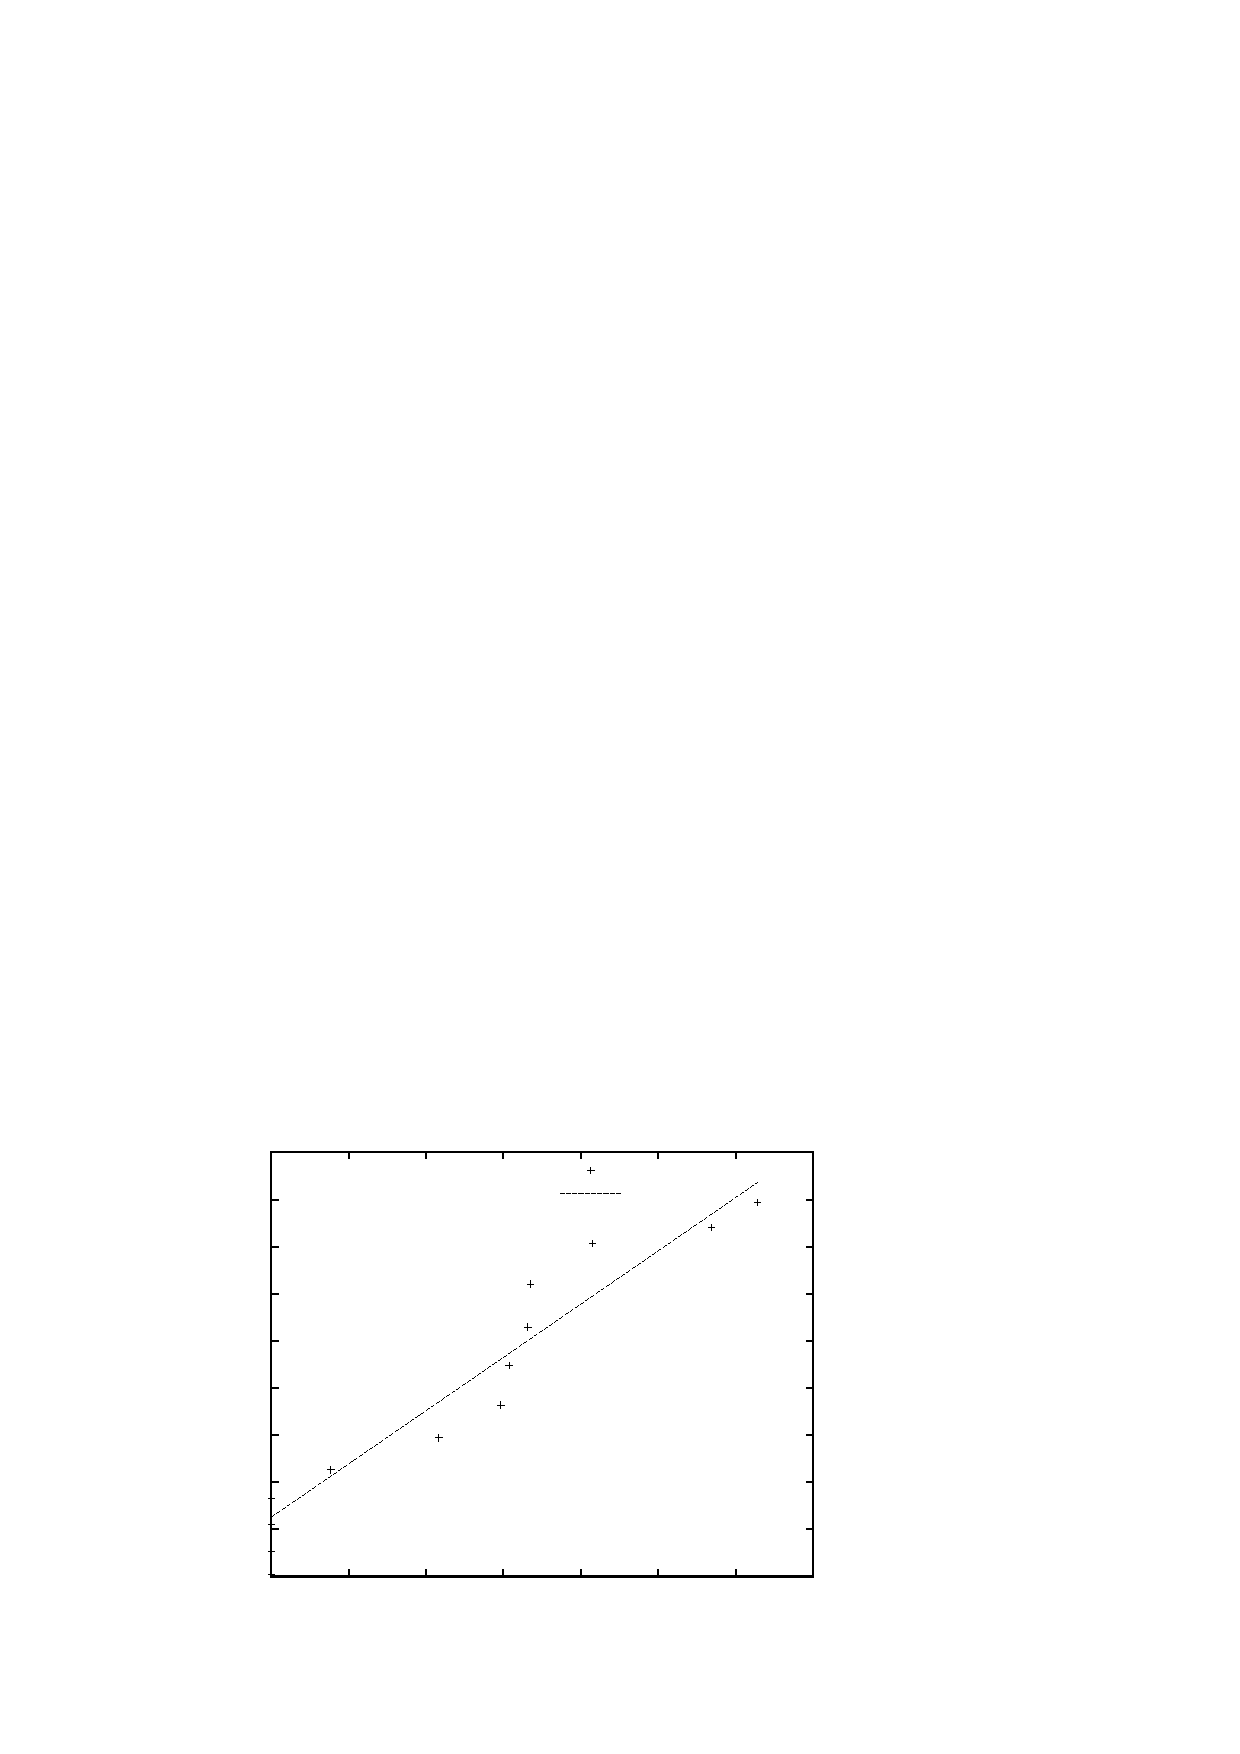
\includegraphics{5a}}%
    \gplfronttext
  \end{picture}%
\endgroup

\end{center}
\caption{Graf závislosti čtverce napětí na posunutí fáze pro první měření za pomoci analyzátoru.}
\label{5a}
\end{figure}


\begin{figure}
\begin{center}
% GNUPLOT: LaTeX picture with Postscript
\begingroup
  \makeatletter
  \providecommand\color[2][]{%
    \GenericError{(gnuplot) \space\space\space\@spaces}{%
      Package color not loaded in conjunction with
      terminal option `colourtext'%
    }{See the gnuplot documentation for explanation.%
    }{Either use 'blacktext' in gnuplot or load the package
      color.sty in LaTeX.}%
    \renewcommand\color[2][]{}%
  }%
  \providecommand\includegraphics[2][]{%
    \GenericError{(gnuplot) \space\space\space\@spaces}{%
      Package graphicx or graphics not loaded%
    }{See the gnuplot documentation for explanation.%
    }{The gnuplot epslatex terminal needs graphicx.sty or graphics.sty.}%
    \renewcommand\includegraphics[2][]{}%
  }%
  \providecommand\rotatebox[2]{#2}%
  \@ifundefined{ifGPcolor}{%
    \newif\ifGPcolor
    \GPcolorfalse
  }{}%
  \@ifundefined{ifGPblacktext}{%
    \newif\ifGPblacktext
    \GPblacktexttrue
  }{}%
  % define a \g@addto@macro without @ in the name:
  \let\gplgaddtomacro\g@addto@macro
  % define empty templates for all commands taking text:
  \gdef\gplbacktext{}%
  \gdef\gplfronttext{}%
  \makeatother
  \ifGPblacktext
    % no textcolor at all
    \def\colorrgb#1{}%
    \def\colorgray#1{}%
  \else
    % gray or color?
    \ifGPcolor
      \def\colorrgb#1{\color[rgb]{#1}}%
      \def\colorgray#1{\color[gray]{#1}}%
      \expandafter\def\csname LTw\endcsname{\color{white}}%
      \expandafter\def\csname LTb\endcsname{\color{black}}%
      \expandafter\def\csname LTa\endcsname{\color{black}}%
      \expandafter\def\csname LT0\endcsname{\color[rgb]{1,0,0}}%
      \expandafter\def\csname LT1\endcsname{\color[rgb]{0,1,0}}%
      \expandafter\def\csname LT2\endcsname{\color[rgb]{0,0,1}}%
      \expandafter\def\csname LT3\endcsname{\color[rgb]{1,0,1}}%
      \expandafter\def\csname LT4\endcsname{\color[rgb]{0,1,1}}%
      \expandafter\def\csname LT5\endcsname{\color[rgb]{1,1,0}}%
      \expandafter\def\csname LT6\endcsname{\color[rgb]{0,0,0}}%
      \expandafter\def\csname LT7\endcsname{\color[rgb]{1,0.3,0}}%
      \expandafter\def\csname LT8\endcsname{\color[rgb]{0.5,0.5,0.5}}%
    \else
      % gray
      \def\colorrgb#1{\color{black}}%
      \def\colorgray#1{\color[gray]{#1}}%
      \expandafter\def\csname LTw\endcsname{\color{white}}%
      \expandafter\def\csname LTb\endcsname{\color{black}}%
      \expandafter\def\csname LTa\endcsname{\color{black}}%
      \expandafter\def\csname LT0\endcsname{\color{black}}%
      \expandafter\def\csname LT1\endcsname{\color{black}}%
      \expandafter\def\csname LT2\endcsname{\color{black}}%
      \expandafter\def\csname LT3\endcsname{\color{black}}%
      \expandafter\def\csname LT4\endcsname{\color{black}}%
      \expandafter\def\csname LT5\endcsname{\color{black}}%
      \expandafter\def\csname LT6\endcsname{\color{black}}%
      \expandafter\def\csname LT7\endcsname{\color{black}}%
      \expandafter\def\csname LT8\endcsname{\color{black}}%
    \fi
  \fi
  \setlength{\unitlength}{0.0500bp}%
  \begin{picture}(7200.00,5040.00)%
    \gplgaddtomacro\gplbacktext{%
      \csname LTb\endcsname%
      \put(1342,704){\makebox(0,0)[r]{\strut{} 0}}%
      \put(1342,1518){\makebox(0,0)[r]{\strut{} 200000}}%
      \put(1342,2332){\makebox(0,0)[r]{\strut{} 400000}}%
      \put(1342,3147){\makebox(0,0)[r]{\strut{} 600000}}%
      \put(1342,3961){\makebox(0,0)[r]{\strut{} 800000}}%
      \put(1342,4775){\makebox(0,0)[r]{\strut{} 1e+06}}%
      \put(1474,484){\makebox(0,0){\strut{} 0}}%
      \put(2007,484){\makebox(0,0){\strut{} 0.5}}%
      \put(2540,484){\makebox(0,0){\strut{} 1}}%
      \put(3073,484){\makebox(0,0){\strut{} 1.5}}%
      \put(3606,484){\makebox(0,0){\strut{} 2}}%
      \put(4138,484){\makebox(0,0){\strut{} 2.5}}%
      \put(4671,484){\makebox(0,0){\strut{} 3}}%
      \put(5204,484){\makebox(0,0){\strut{} 3.5}}%
      \put(5737,484){\makebox(0,0){\strut{} 4}}%
      \put(6270,484){\makebox(0,0){\strut{} 4.5}}%
      \put(6803,484){\makebox(0,0){\strut{} 5}}%
      \put(176,2739){\rotatebox{-270}{\makebox(0,0){\strut{}$(U/\mbox{V})^2$}}}%
      \put(4138,154){\makebox(0,0){\strut{}$\Delta/\mbox{rad}$}}%
    }%
    \gplgaddtomacro\gplfronttext{%
      \csname LTb\endcsname%
      \put(4114,4602){\makebox(0,0)[r]{\strut{}naměřené hodnoty}}%
      \csname LTb\endcsname%
      \put(4114,4382){\makebox(0,0)[r]{\strut{}f(x)}}%
    }%
    \gplbacktext
    \put(0,0){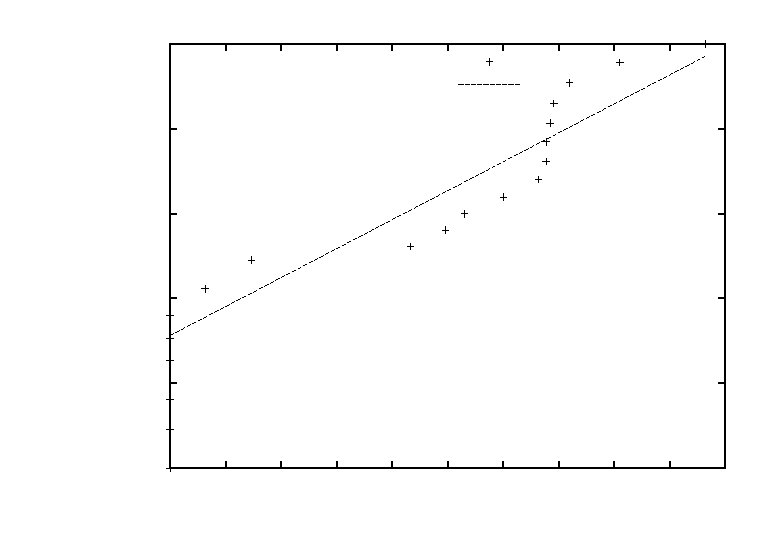
\includegraphics{5b}}%
    \gplfronttext
  \end{picture}%
\endgroup

\end{center}
\caption{Graf závislosti čtverce napětí na posunutí fáze pro druhé měření za pomoci analyzátoru.}
\label{5b}
\end{figure}

\begin{figure}
\begin{center}
% GNUPLOT: LaTeX picture with Postscript
\begingroup
  \makeatletter
  \providecommand\color[2][]{%
    \GenericError{(gnuplot) \space\space\space\@spaces}{%
      Package color not loaded in conjunction with
      terminal option `colourtext'%
    }{See the gnuplot documentation for explanation.%
    }{Either use 'blacktext' in gnuplot or load the package
      color.sty in LaTeX.}%
    \renewcommand\color[2][]{}%
  }%
  \providecommand\includegraphics[2][]{%
    \GenericError{(gnuplot) \space\space\space\@spaces}{%
      Package graphicx or graphics not loaded%
    }{See the gnuplot documentation for explanation.%
    }{The gnuplot epslatex terminal needs graphicx.sty or graphics.sty.}%
    \renewcommand\includegraphics[2][]{}%
  }%
  \providecommand\rotatebox[2]{#2}%
  \@ifundefined{ifGPcolor}{%
    \newif\ifGPcolor
    \GPcolorfalse
  }{}%
  \@ifundefined{ifGPblacktext}{%
    \newif\ifGPblacktext
    \GPblacktexttrue
  }{}%
  % define a \g@addto@macro without @ in the name:
  \let\gplgaddtomacro\g@addto@macro
  % define empty templates for all commands taking text:
  \gdef\gplbacktext{}%
  \gdef\gplfronttext{}%
  \makeatother
  \ifGPblacktext
    % no textcolor at all
    \def\colorrgb#1{}%
    \def\colorgray#1{}%
  \else
    % gray or color?
    \ifGPcolor
      \def\colorrgb#1{\color[rgb]{#1}}%
      \def\colorgray#1{\color[gray]{#1}}%
      \expandafter\def\csname LTw\endcsname{\color{white}}%
      \expandafter\def\csname LTb\endcsname{\color{black}}%
      \expandafter\def\csname LTa\endcsname{\color{black}}%
      \expandafter\def\csname LT0\endcsname{\color[rgb]{1,0,0}}%
      \expandafter\def\csname LT1\endcsname{\color[rgb]{0,1,0}}%
      \expandafter\def\csname LT2\endcsname{\color[rgb]{0,0,1}}%
      \expandafter\def\csname LT3\endcsname{\color[rgb]{1,0,1}}%
      \expandafter\def\csname LT4\endcsname{\color[rgb]{0,1,1}}%
      \expandafter\def\csname LT5\endcsname{\color[rgb]{1,1,0}}%
      \expandafter\def\csname LT6\endcsname{\color[rgb]{0,0,0}}%
      \expandafter\def\csname LT7\endcsname{\color[rgb]{1,0.3,0}}%
      \expandafter\def\csname LT8\endcsname{\color[rgb]{0.5,0.5,0.5}}%
    \else
      % gray
      \def\colorrgb#1{\color{black}}%
      \def\colorgray#1{\color[gray]{#1}}%
      \expandafter\def\csname LTw\endcsname{\color{white}}%
      \expandafter\def\csname LTb\endcsname{\color{black}}%
      \expandafter\def\csname LTa\endcsname{\color{black}}%
      \expandafter\def\csname LT0\endcsname{\color{black}}%
      \expandafter\def\csname LT1\endcsname{\color{black}}%
      \expandafter\def\csname LT2\endcsname{\color{black}}%
      \expandafter\def\csname LT3\endcsname{\color{black}}%
      \expandafter\def\csname LT4\endcsname{\color{black}}%
      \expandafter\def\csname LT5\endcsname{\color{black}}%
      \expandafter\def\csname LT6\endcsname{\color{black}}%
      \expandafter\def\csname LT7\endcsname{\color{black}}%
      \expandafter\def\csname LT8\endcsname{\color{black}}%
    \fi
  \fi
  \setlength{\unitlength}{0.0500bp}%
  \begin{picture}(7200.00,5040.00)%
    \gplgaddtomacro\gplbacktext{%
      \csname LTb\endcsname%
      \put(1342,704){\makebox(0,0)[r]{\strut{} 200000}}%
      \put(1342,1213){\makebox(0,0)[r]{\strut{} 300000}}%
      \put(1342,1722){\makebox(0,0)[r]{\strut{} 400000}}%
      \put(1342,2231){\makebox(0,0)[r]{\strut{} 500000}}%
      \put(1342,2740){\makebox(0,0)[r]{\strut{} 600000}}%
      \put(1342,3248){\makebox(0,0)[r]{\strut{} 700000}}%
      \put(1342,3757){\makebox(0,0)[r]{\strut{} 800000}}%
      \put(1342,4266){\makebox(0,0)[r]{\strut{} 900000}}%
      \put(1342,4775){\makebox(0,0)[r]{\strut{} 1e+06}}%
      \put(1474,484){\makebox(0,0){\strut{} 0}}%
      \put(2140,484){\makebox(0,0){\strut{} 0.5}}%
      \put(2806,484){\makebox(0,0){\strut{} 1}}%
      \put(3472,484){\makebox(0,0){\strut{} 1.5}}%
      \put(4139,484){\makebox(0,0){\strut{} 2}}%
      \put(4805,484){\makebox(0,0){\strut{} 2.5}}%
      \put(5471,484){\makebox(0,0){\strut{} 3}}%
      \put(6137,484){\makebox(0,0){\strut{} 3.5}}%
      \put(6803,484){\makebox(0,0){\strut{} 4}}%
      \put(176,2739){\rotatebox{-270}{\makebox(0,0){\strut{}$(U/\mbox{V})^2$}}}%
      \put(4138,154){\makebox(0,0){\strut{}$\Delta/\mbox{rad}$}}%
    }%
    \gplgaddtomacro\gplfronttext{%
      \csname LTb\endcsname%
      \put(4114,4602){\makebox(0,0)[r]{\strut{}naměřené hodnoty}}%
      \csname LTb\endcsname%
      \put(4114,4382){\makebox(0,0)[r]{\strut{}f(x)}}%
    }%
    \gplbacktext
    \put(0,0){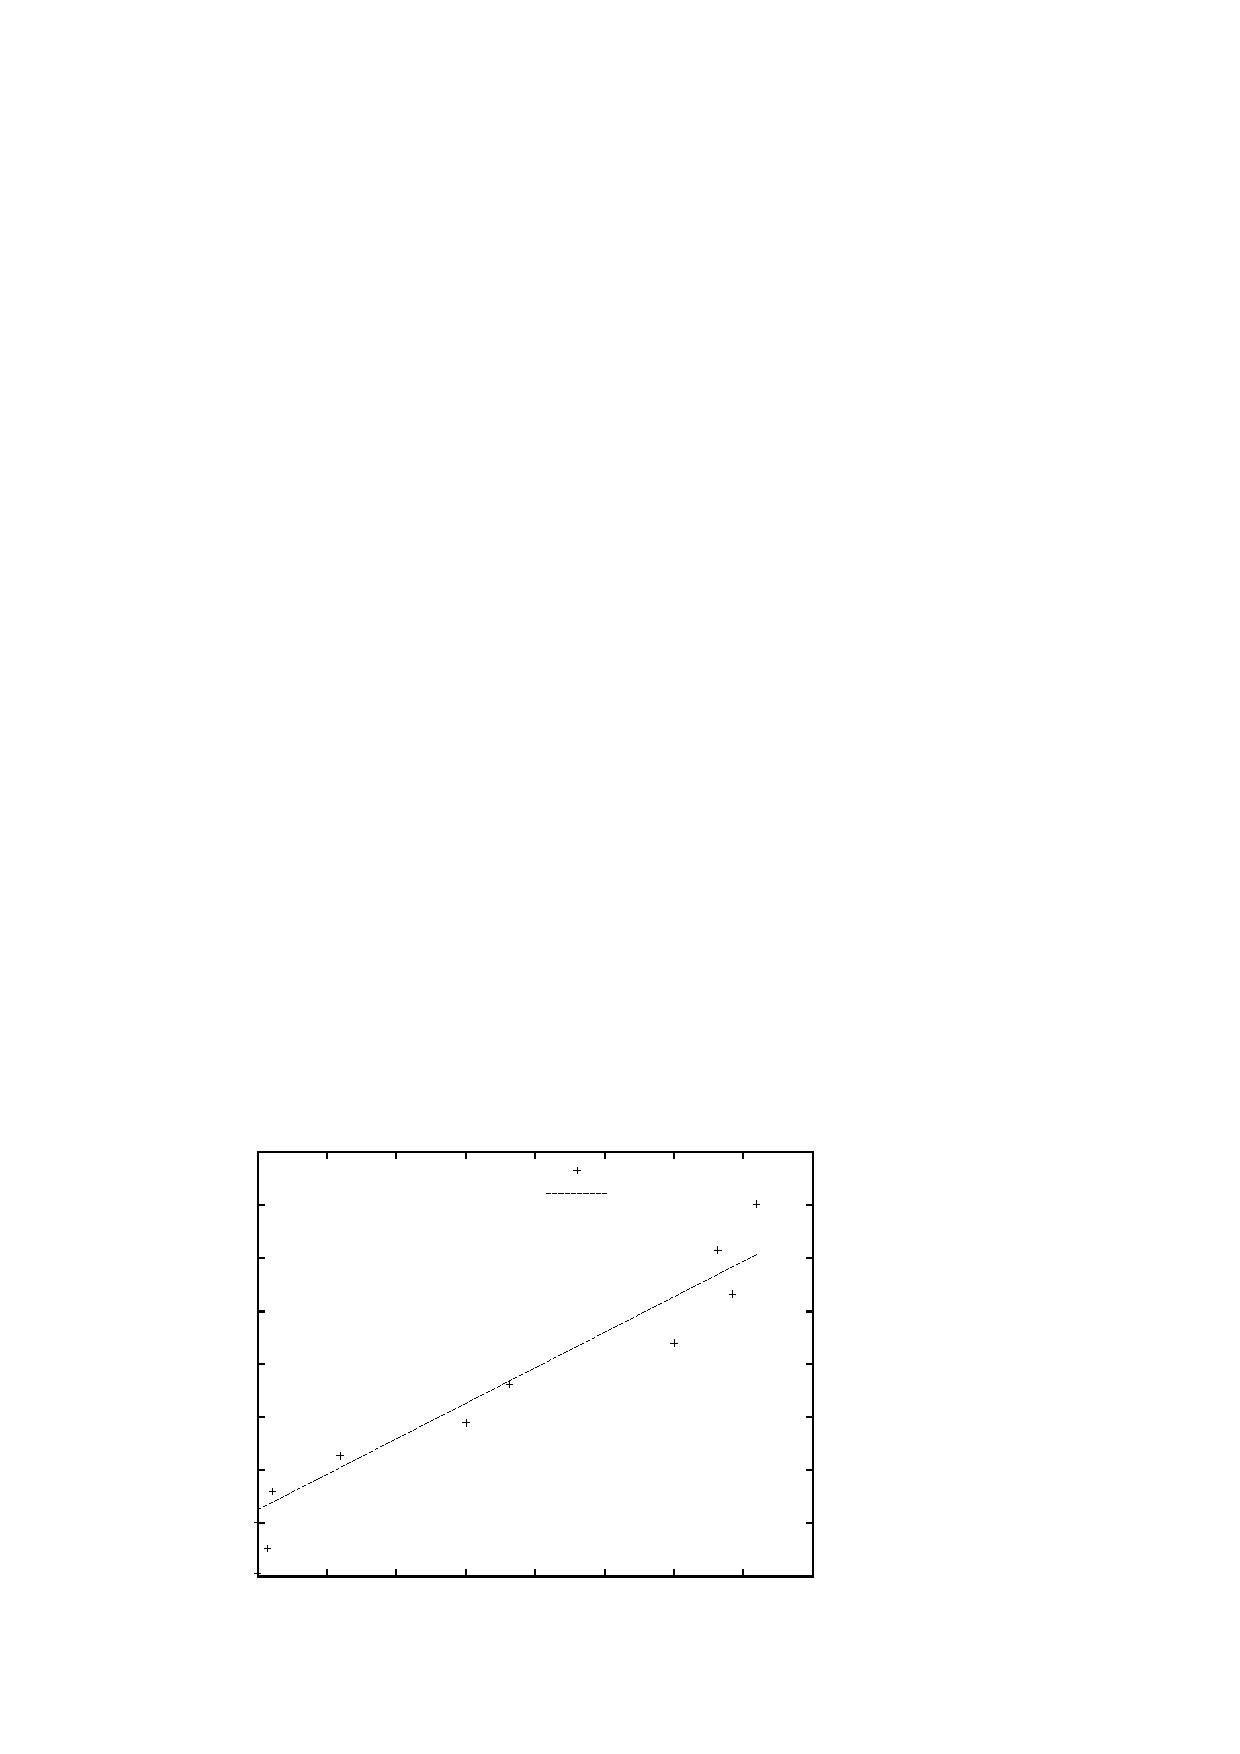
\includegraphics{5c}}%
    \gplfronttext
  \end{picture}%
\endgroup

\end{center}
\caption{Graf závislosti čtverce napětí na posunutí fáze pro třetí měření za pomoci analyzátoru.}
\label{5c}
\end{figure}

\section{Diskuze}
\subsection{Vliv vnějšího světla}
Po proměření intenzit pro různé světelné podmínky v místnosti, konkrétně intenzita světla z oken, vnitřní osvětlení, stínění osob v místnosti, jsem dospěl 
k názoru, že pro měření není potřeba zatemněná místnost. Posunuí nulové hodnoty intenzity bylo způsobeno polohou nastavenou na fotonásobiči. Rozdíl mezi zatemněnou 
místností byl v rámci chyby určení intenzity. Jako poslední jsem pozoroval vliv lampičky u vedlejěího stolu při zatemněné místosti, kdy se intenzita na detektoru 
po jijím rozsvícení vůbec nezmněnila.

\subsection{Poloha polarizačních filtrů}
Při zjišťování snadného směru průchodu polarizátoru jsem uvedl, že nepřesnot byla okolo $3\st$. Celé rozložení však mělo poněkud improvizovaný charakter. Filtr nebyl 
umístěný v držáku, úhel sklíčka byl nastaven pouze přibližně a zdrojem světla byla lampa, která se ne příliš lehce nastavovala do kýřené polohy. Proto si myslím, že 
nulová poloha polarizačního filtru byla mnohem přesnější, než je uvedeno výše.

Z tohoto důvodu jsem považoval zkřížení polarizátorů téměř bez chyby, čemuž odpovídalo i pozorování při různých polohách filtrů. 

\subsection{Kerrova konstanta určená za pomoci intenzity při zkřížených polarizátorech}
\subsubsection{Fitování na závislost intenzity na napětí}
Jak bylo uvedeno výše, abych dospěl k fitu, který odpovídá naměřeným hodnotám a jeho chyba je nižší než 20 \%, musel jsem do teoretické závislosti přidat faktor, 
který by odpovídal tomu, že vzorek vůbec nereaguje na malá napětí. U tohoto fitování byla hodnota tohoto posunu určena spíše zkusmo tak, aby fit měl co nejmenší chybu, 
protože program gnuplot si tuto hodnotu sám neposunul. Druhé měření se potom ukázalo o něco přesnější. Při relaxační době 30 s totiž bylo mnohdy vidět, že 
se velikost intenzity má stále tendenci měnit, především při poklesu z maxima. K ustálení většinou docházelo okolo 45 s. Dále značně pomohlo zkrácení kroku.

\subsubsection{Fit na závislost kvadrátu na fázovém posunu}
Tento fit byl mnohem lepší z hlediska přesnosti určení napětí, od kdy přibližně začíná vzorek reagovat, protože gnuplot mnohem lépe pracoval s lineární funkcí, kde 
byly pouze dvě volné konstanty. Jediný problím nastal u výpočtu fázového posunu, kdy jsem zvolil maximum jako hodnotu určenou z předešlého fitu. Vypočítaná Kerrova 
konstanta následně vyšla o něco menší a považuji je za něco přesnější, ač mají stejnou chybu, jako ty určené předchozí metodou.

\subsection{Kerrova konstanta určena z fázového posunu určeného za pomoci analyzátoru}
Tato metoda se zpracovávala stejně jako ta uvedená výše, což bylo dobré z hlediska fitu. Problém byl však s přesným určením fázového posunu. Během měření se 
objevili jevy které mohli mít vliv i na předchozí měření. První problém byl při určení minima intenzity. Toto minimum totiž bylo velmi mělké. Rozptyl jsem odhadl 
pro menší zesílení na $4\st$. Větší zesílení bylo asi dvakrát přesnější. Další problém byl spoždění hodnoty na voltmetru. Tento jev se dal upravovat integrační 
dobou fotonásobiče. Zkoušel jsem použít větší hodnotu (3 s), abych vyloučil fluktuace intenzity, ale to i při posunu analyzátoru vždy po 3 sekundách lokalizace 
minima nepomohlo. Časovou konstantu jsem proto nakonec použil co nejmenší. Obtíže také nastali, když jsem minimum přejel a začal se vracet. Intenzita mnohdy při 
pohybu na druhou stranu poskočila. Podobný jev nastal při zastavení a opětovném posunu analyzátoru. Dále jsem zaznamenal více minim pro stejnou hodnotu napětí na 
vzorku. Při bližším zkoumání tohoto jevu jsem si povšiml, že jsou některá z těchto minim nezávislá na nastaveném napětí. Nejvýraznější bylo u $0\st$ a $90\st$ na analyzátoru. 
Z tohoto důvodu bylo měření v okolí těchto bodů obtížnější, protože tato minima se překrývala s minimy způsobenými Kerrovým jevem. Předpokládám, že tento problém 
vznikl následkem různých odrazů. Nejvýraznější vznikal na držáku vzorkum jehož obraz byl pozorovatelný jako výrazná šmouha na polarizátoru.

Výsledky získané touto metodou se v rámci chyby téměř schodují s výsledky první metody. Nižší hodnota Kerrovy konstanty je pravděpodobna způsobena delší dobou odečítání 
úhlu z analyzátoru. Celková chyba je však kvůli jevům uvedeným výše o řád vyšší.

\subsection{Vliv nepřesnosti parametrů $d$ a $l$}
Parametry $d$ a $l$ byly zadány bez jakékoliv chyby. Proto tato chyba nemohl být započítána do výsledků a je brána za zanedbatelnou. Abych tak mohl bez potíží 
učinit, musí být relativní chyba o řád nižší než nejvyšší nepřesnost vyskytující se ve vzorcích. Vzhledem k výskytu $d$ ve druhé mocnině musí být její relativní chyba 
ještě menší. Veličinou k porovnání je zpravidla naměřená intenzita. Její chyba se pohybuje v řádu procent. To by znamenalo měřit $l$ s přesností na mikrometry a lépe, 
v případě $d$ spíše desetiny mikrometrů. Tato přesnost je za použití například mikroskopu dosažitelná, avšak u parametrů není uveden ani způsob jejich určení. Za předpokladu, 
že jsou parametry určeny s přesností na jejich poslední platnou číslici by chyba byla o řád vyšší.

\section{Závěr}
Sestavil jsem aparaturu pro měření Kerrova jevu v pevné látce. \\
Změřil jsem závislost intenzity světla dopadajícího na detektor na napětí přiloženém na elektrody vzorku. Data jsou v tabulkách \ref{TM30} a \ref{TM60}. Grafické zpracování 
je na obrázcích \ref{G30} a \ref{G60}. \\
Za pomoci fitů na zavislost intenzity na napětí a závislosti kvadrátu napětí na fázovém posunu jsem stanovil Kerrovu konstantu
\begin{eqnarray}
K_{30}&=&(4.5\pm0.1)\cdot 10^{-9} \mbox{m}/\mbox{V}^2\\
K_{60}&=&(4.12\pm0.06)\cdot 10^{-9} \mbox{m}/\mbox{V}^2 \\
K_{30b}&=&(4.0\pm0.1)\cdot 10^{-9}\mbox{m}/\mbox{V}^2 \\
K_{60b}&=&(3.65\pm0.06)\cdot 10^{-9}\mbox{m}/\mbox{V}^2 
\end{eqnarray}
Vypočetl jsem půlvnné napětí
\begin{eqnarray}
U_{\lambda/2}=1020\pm 20 \mbox{V}
\end{eqnarray}
Diskutoval jsem vliv nepřesnoti zadaných parametrů na přesnost výsledků. \\
Změřil jsem závislost fázového posunu na napětí na vzorku za pomoci proměnné polohy analyzátoru. Výsledky jednotlivých měření jsou v tabulkách \ref{T5a}, \ref{T5b} a \ref{T5c}. 
Grafy závislotí jsou na obrázcích \ref{5a}, \ref{5b} a \ref{5c}. \\
Dopočtné Kerrovy konstanty jsou
\begin{eqnarray}
K_{5a}&=&(3.6\pm 0.6) \cdot 10^{-9} \mV \\
K_{5b}&=&(3.0\pm0.4) \cdot 10^{-9} \mV \\
K_{5c}&=&(3.1\pm0.4) \cdot 10^{-9} \mV
\end{eqnarray}



\begin{thebibliography}{5}
	\bibitem{text} \textbf{Studijní text na praktikum III} \\http://physics.mff.cuni.cz/vyuka/zfp/txt\_327.htm (24. 3. 2012)
    \bibitem{chyba} \emph{J. Englich}: \textbf{Zpracování výsldků fyzikálních měření} \\ LS 1999/2000
    \bibitem{maly} \emph{prof. RNDr. Petr Malý , DrSc.}: \textbf{Optika}\\Univerzita Karlova v Praze, Nakladatelství Karolinum 2008, první vydání
\end{thebibliography}




\end{document}
